\documentclass[11pt,letterpaper]{article}

\usepackage[T1]{fontenc}
\usepackage[utf8]{inputenc}
\usepackage{mathpazo}
\usepackage[scaled=0.95]{helvet}
\usepackage{courier}
\linespread{1.04}
\usepackage{microtype}
\usepackage[margin=1in]{geometry}
\usepackage{amsmath,amssymb,mathtools}
\usepackage{booktabs,longtable,tabularx,array}
\usepackage{enumitem}
\usepackage[dvipsnames]{xcolor}
\usepackage{tikz}
\usetikzlibrary{arrows.meta,positioning,shapes.geometric}
\usepackage{fancyhdr}
\usepackage{parskip}
\usepackage[strings]{underscore}
\usepackage{xurl}
\usepackage[colorlinks=true,linkcolor=MidnightBlue,urlcolor=MidnightBlue,citecolor=MidnightBlue]{hyperref}

\emergencystretch=3em
\setlength{\headheight}{14pt}

% ---------- macros ----------
\newcommand{\code}[1]{\texttt{#1}}
\newcommand{\E}{\mathbb{E}}
\newcommand{\ind}[1]{\mathbf{1}\!\left[#1\right]}
\newcommand{\bp}{\,\mathrm{bp}}
\newcommand{\Pm}{\bar{P}}                 % mid price
\newcommand{\hs}{\mathrm{hs}}             % half-spread
\newcommand{\ADV}{\mathrm{ADV}}
\newcommand{\SD}{\mathrm{SD}}             % spread duration
\newcommand{\rres}{r^{\mathrm{res}}}      % residual return
\newcommand{\rcx}{r^{\mathrm{cx}}}        % credit excess return
\newcommand{\Imb}{\mathrm{Imb}}
\newcommand{\FIT}{\mathrm{FIT}}
\newcommand{\Neff}{N_{\mathrm{eff}}}
\makeatletter
\newcommand*{\twodigit}[1]{\expandafter\@twodigit\csname c@#1\endcsname}
\newcommand*{\@twodigit}[1]{\ifnum#1<10 0\fi\number#1}
\AddEnumerateCounter{\twodigit}{\@twodigit}{00}
\makeatother

% step lists: \begin{ladder}[label=\textbf{A1.\twodigit*}] ... \end{ladder}
\newlist{ladder}{enumerate}{1}
\setlist[ladder]{leftmargin=4.4em,labelsep=0.6em,itemsep=3pt,topsep=4pt}
\newcommand{\stepname}[1]{\textbf{#1.}}
\newcommand{\Out}{\textit{Output:}~}
\newcommand{\Pass}{\textit{Pass:}~}

% signal specification blocks
\newlist{spec}{description}{1}
\setlist[spec]{leftmargin=1.4em,labelsep=0.5em,itemsep=3pt,topsep=4pt,font=\normalfont\bfseries}

\pagestyle{fancy}
\fancyhf{}
\lhead{\small Twenty Signals for Residualised Corporate Bond Returns}
\rhead{\small \thepage}
\renewcommand{\headrulewidth}{0.3pt}

\title{\textbf{Twenty Signals for Residualised Corporate Bond Returns\\ at 5- and 10-Day Horizons}\\[6pt]
\large Thesis, signal specifications, adversarial review,\\ and agent implementation playbook}
\author{Working document, version 3\\ \small regenerated after a second line-by-line audit}
\date{18 September 2026}

\begin{document}
\maketitle
\thispagestyle{fancy}

\begin{abstract}
\noindent
This document specifies twenty signals for predicting residualised corporate bond returns over 5 and 10 business days, and the conditions under which they can be monetised net of transaction costs. Its central claim is deliberately narrow. No signal and no gate makes every trade cover its cost. What can be built and verified is a quoting book whose long-run mean net markout per opportunity stays at or above a small tolerance below zero, with failures budgeted for liquidity stress. The edge is a structural advantage (flow information, cost and outlet, repricing latency); the signals only aim it.

Part~I states the thesis, the three return targets, the cost model and the risk-controlled gate. Part~II specifies the twenty signals in five families, their combination into a single fill-conditional markout, and the validation protocol with five pre-registered kill tests. Part~III records the three-loop adversarial review that narrowed the original claim. Part~IV is an agent implementation playbook: twelve operating rules, a prompt wrapper, twenty-four shared foundation steps, an eight-step standard tail, and twenty signal ladders totalling 181 build steps, each starting from data discovery. Appendix~A logs every correction made in the two audits, so that a reader of an earlier version can see exactly what changed.
\end{abstract}

\tableofcontents
\newpage
\part{Thesis and measurement}

\section{Thesis: the edge is a structural advantage, and signals only aim it}
\label{sec:thesis}

No signal and no gate makes every trade cover its cost. What can be built and verified is narrower: a quoting book whose long-run mean net markout per opportunity stays at or above a small tolerance below zero, with failures budgeted for liquidity stress. This statement survived three rounds of adversarial review (Part~III) and two line-by-line audits (Appendix~\ref{app:audit}).

\subsection{Equilibrium first}
Gross predictability in corporate bonds is roughly the marginal arbitrageur's cost of harvesting it. Public data plus spread-crossing therefore nets to zero. That is what Dickerson, Nozawa and Robotti \cite{dnr2024} find: machine-learning bond strategies earn zero or negative bond-CAPM alpha once bid-ask spreads and execution delays are charged. Positive net edge needs an advantage that the marginal participant lacks. A dealer desk has three:
\begin{enumerate}[itemsep=2pt,topsep=2pt]
\item \textbf{Flow information:} its own RFQ traffic and fills, which no TRACE-only researcher can see.
\item \textbf{Cost and outlet:} spread that is earned rather than paid, and cheap exits through client flow, ETF creation and redemption, and portfolio-trade recycling.
\item \textbf{Repricing latency:} the ability to reprice mechanically (for example after a Treasury move) before rivals do.
\end{enumerate}

\subsection{The taker hurdle still binds}
Let $z$ be a standardised signal, $r$ the residual return over horizon $h$ with standard deviation $\sigma_h$, and $\mathrm{IC}=\mathrm{corr}(z,r)$. Under joint normality
\begin{equation}
\E[r \mid z] \;=\; \mathrm{IC}\,\sigma_h\, z .
\end{equation}
Crossing a round-trip cost $c$ is worthwhile only when
\begin{equation}
z \;>\; z^{*} \;=\; \frac{c}{\mathrm{IC}\,\sigma_h}.
\label{eq:zstar}
\end{equation}
With $\mathrm{IC}=0.05$, $\sigma_{10d}=60\bp$ and $c=25\bp$, $z^{*}=25/(0.05\times 60)=8.3$. A weak public signal never trades as a liquidity taker, however clean its backtest $t$-statistic.

\subsection{Accounting identity}
For a fill at price $p$ against the contemporaneous mid $\Pm_t$, with $s=+1$ when the desk buys and $s=-1$ when it sells,
\begin{equation}
\mathrm{PnL}_h \;=\; \underbrace{s\,(\Pm_t - p)}_{\text{spread capture}} \;+\; \underbrace{s\,(\Pm_{t+h}-\Pm_t)}_{\text{markout } \mathcal{M}_h} \;-\; c ,
\label{eq:identity}
\end{equation}
where $c$ collects exit, hedge and funding costs (Section~\ref{sec:cost}). The first term belongs to the franchise. Signals are credited only with the second term, measured mid to mid and conditional on the fill. This removes the double count between earned spread and ``reversal alpha'' that an earlier version of this document contained.

\subsection{The decision is a quote, not a trade}
Consider a bid at offset $d$ below mid, so the bid is $\Pm_t-d$. Let $W(d\mid x)$ be the probability of winning the RFQ given features $x$, decreasing in $d$, and let
\[
m(d,x) \;=\; \E\!\left[\mathcal{M}_h \,\middle|\, \text{win at offset } d,\; x\right]
\]
be the \emph{fill-conditional} expected markout. Expected profit per RFQ is
\begin{equation}
\Pi(d) \;=\; W(d\mid x)\,\bigl[\,d + m(d,x) - c\,\bigr].
\label{eq:quote}
\end{equation}
Differentiating, $\Pi'(d)=W'(d)\,[d+m-c]+W(d)\,[1+m'(d)]=0$, and since $W'<0$,
\begin{equation}
d^{*} \;=\; \frac{W(d^{*})}{|W'(d^{*})|}\,\bigl(1+m'(d^{*})\bigr) \;-\; m(d^{*},x) \;+\; c .
\label{eq:foc}
\end{equation}
Four remarks.
\begin{enumerate}[itemsep=2pt,topsep=2pt]
\item The first term is the inverse-hazard markup of the hit-ratio quoting problem in the RFQ market-making literature \cite{hitratio2026,bg2023}. The twenty signals matter only through $m$.
\item $m$ is conditional on winning. A passive bid that still wins means every rival bid lower, which is bad news, so $m$ falls as $d$ rises and $m'(d)<0$. The skew equals the fill-conditional markout, never the unconditional forecast.
\item At the optimum, expected net P\&L per fill is $d^{*}+m-c=(W/|W'|)(1+m')$, which is positive whenever $1+m'>0$.
\item The offer side is symmetric: an offer at $\Pm_t+d_a$ earns $d_a+m_a-c$ when lifted, with $m_a=\E[-(\Pm_{t+h}-\Pm_t)\mid \text{win}]$.
\end{enumerate}

\paragraph{Taker execution as a boundary case.}
Crossing the street's spread corresponds to $d=-\hs^{\mathrm{street}}$ with $W=1$. It is worth it only when $m-c>\hs^{\mathrm{street}}$, which is the hurdle~\eqref{eq:zstar} again. Whether to cross now or wait for a maker fill depends on how fast the signal decays. Let right-side RFQs arrive at rate $\nu$ per day, be won with probability $W$, and let the unconditional markout decay as $m_0\,2^{-\theta/T_{1/2}}$ with waiting time $\theta$. With $a=\nu W$ and $\beta=\ln 2/T_{1/2}$, the value of waiting up to $T$ days is
\begin{equation}
V^{\mathrm{maker}} \;=\; (d-c)\bigl(1-e^{-aT}\bigr) \;+\; m_0\,\frac{a}{a+\beta}\bigl(1-e^{-(a+\beta)T}\bigr),
\qquad
V^{\mathrm{taker}} \;=\; m_0-\hs^{\mathrm{street}}-c .
\label{eq:wait}
\end{equation}
Illustration: $\nu=0.15$, $W=0.2$, $T_{1/2}=5$, $T=10$, $d=10\bp$, $c=8\bp$, $\hs^{\mathrm{street}}=15\bp$ give $V^{\mathrm{maker}}=0.52+0.145\,m_0$ and $V^{\mathrm{taker}}=m_0-23$. Crossing wins only when $m_0>27.5\bp$. These inputs are placeholders for the desk's own estimates.

\subsection{Four return sources, not twenty alphas}
\begin{center}
\begin{tabularx}{\textwidth}{@{}l l X X@{}}
\toprule
Source & Signals & Advantage used & Nature \\
\midrule
L: liquidity premium & A1, A2, A4, C1, D2, E1, E2 & Cost and outlet & A risk premium, negatively skewed; sized on a stress scenario \\
I: information diffusion & A5, B1--B5, C2, E3 & Low cost in liquid bonds, nothing more & Closest to alpha, so it faces the hardest tests \\
F: flow information & A3 & Own RFQ traffic & Proprietary; scales with market share \\
M: mechanics and calendars & C3, D1, D3, D4 & Repricing latency and known dates & Small, high hit rate, crowding risk \\
\bottomrule
\end{tabularx}
\end{center}

\subsection{Breadth is capped by correlation, so the guarantee lives in time}
For $N$ equally weighted positions with common volatility $\sigma$ and average pairwise correlation $\bar\rho$,
\begin{equation}
\mathrm{Var}\Bigl(\tfrac1N\textstyle\sum_i r_i\Bigr)=\sigma^2\Bigl[\tfrac1N+\bigl(1-\tfrac1N\bigr)\bar\rho\Bigr]
\quad\Longrightarrow\quad
\Neff=\frac{N}{1+(N-1)\bar\rho}\;\le\;\frac{1}{\bar\rho}.
\label{eq:neff}
\end{equation}
At $\bar\rho=0.05$ the cap is 20, so $\sigma_{\mathrm{book}}=60/\sqrt{20}=13.4\bp$. A $5\bp$ net edge is then a per-window Sharpe ratio of $0.37$, and only about $64\%$ of windows are positive. No single window can be guaranteed. Over about 25 ten-day windows a year the Sharpe ratio is near $0.37\sqrt{25}\approx1.9$, a roughly $97\%$ chance of a positive year if windows were independent. Stress clustering lowers that figure, which is why the liquidity source is sized on a stress scenario (Section~\ref{sec:cost}).

\section{Notation}
\begin{center}
\begin{longtable}{@{}p{0.2\textwidth}p{0.75\textwidth}@{}}
\toprule
Symbol & Meaning \\
\midrule
\endhead
$i$, $j(i)$, $b(i)$ & Bond, its issuer, its bucket (sector, rating, maturity or liquidity as stated) \\
$t$, $h$ & Business day; horizon in business days, $h\in\{5,10\}$ \\
$\Pm_t$, $p$ & Mid price proxy; fill price \\
$s$, $s^{c}$ & Desk side ($+1$ buy); customer side ($+1$ customer buy) \\
$d$, $W$, $m$ & Quote offset from mid; win probability; fill-conditional expected markout \\
$\mathcal{M}_h$ & Realised markout $s(\Pm_{t+h}-\Pm_t)$ \\
$c$ & Exit, hedge, basis-risk and funding cost, in bp of price \\
$\hs$, $\widehat{\hs}$ & Half-spread; its estimate by bond, size bucket and month (\code{h_hat} in code) \\
$\rcx$, $\rres$ & Credit excess return; cross-sectional residual return \\
$r(t-k,t)$ & Return from the close of $t-k$ to the close of $t$, i.e.\ over days $t-k+1,\dots,t$ \\
$\mathrm{IC}$, $\sigma_h$, $z$ & Information coefficient; residual volatility at horizon $h$; standardised score \\
$I_{i,t}$ & Five-day net dealer purchases from customers over amount outstanding \\
$\kappa$ & Block concession in bp, relative to the pre-trade mid and net of the bucket move \\
$\nu^{\pm}$, $\Imb$ & Decayed counts of client buy and sell inquiries; their imbalance \\
$\beta^{E}$ & Bond's empirical hedge ratio to issuer equity (\code{beta_E}) \\
$\SD$, $\mathrm{ED}^{(k)}$ & Spread duration; empirical rates duration measured at a $k$-day horizon \\
$b$, $\varphi$ & C1 pressure coefficient; C1 level weight \\
$w^{\mathrm{liq}}$ & E1 pecking-order weight (\code{w_liq}) \\
$\lambda$, $\alpha$, $\delta$, $\eta$ & Gate threshold; risk level; confidence parameter; online step size \\
$k_i$ & Price-impact coefficient in the cost function \\
$\gamma$ & Inventory risk aversion in the quote shift \\
$\bar\rho$, $\Neff$ & Average pairwise correlation of position P\&L; effective breadth \\
\bottomrule
\end{longtable}
\end{center}

\section{Targets: three versions of the 5- and 10-day return}
\label{sec:targets}

Signals are researched on a statistical residual, paid on a tradable residual, and sized on a fill-conditional markout. All three are mid to mid, in bp of price, so that bid-ask bounce and stale marks cannot pass as alpha.

\begin{enumerate}[itemsep=4pt]
\item \textbf{Mid proxy, not last trade.} Use the inter-dealer VWAP when it exists. Otherwise average the customer-buy and customer-sell VWAPs. Otherwise side-adjust the print, $\Pm = P - s^{c}\,\widehat{\hs}$, with $s^{c}=+1$ for a customer buy. Drop trades under \$100k and down-weight portfolio-trade prints.

\item \textbf{Credit excess return.} $\rcx$ is total return less a key-rate-matched Treasury return. For HY use empirical, spread-dependent duration. At index level the rates and credit components correlate at $-6.7\%$ in IG and $-34.7\%$ in HY \cite{andreani2024}, so an analytical hedge leaks rates into the residual.

\item \textbf{Statistical residual, for research.} Each date run the cross-sectional regression
\begin{equation}
\rcx_i(t+1,\,t+1+h) \;=\; a_t + b_t\,\mathrm{DTS}_{i,t} + \sum_k c_{k,t}\,\ind{i\in k} + \rres_i(t+1,\,t+1+h),
\end{equation}
with $k$ running over sector-by-rating, maturity and liquidity buckets, all measured at $t$. The target is $y(i,t,h)=\rres_i(t+1,t+1+h)$: the signal is stamped at the close of $t$ and entry is one day later. DTS carries the market beta because spread moves scale with spread level. The same code produces the \emph{trailing} panel $\rres_i(t-k,t)$ for $k\in\{1,5,10,21\}$, which several signals use as an input. The statistical residual ranks signals. It cannot be hedged, so it overstates capturable edge.

\item \textbf{Tradable residual, for P\&L.} Residualise against instruments only,
$r^{\mathrm{res,trd}}_i=\rcx_i-\sum_j\hat\beta_{ij,t-1}f_j$, with $f_j$ the returns of CDX IG or HY, LQD or HYG where cheaper, and Treasury futures by key rate. Charge hedge cost and a cash-index basis risk charge to the position. A signal that lives only in the statistical residual is not monetisable.

\item \textbf{Fill-conditional markout, for sizing.} $\mathcal{M}_h=s(\Pm_{t+h}-\Pm_t)$ from the fill time. Measure it on the desk's wins. For RFQs the desk lost, measure it at the winning price printed on TRACE. This is the $m(d,x)$ of~\eqref{eq:quote}.

\item \textbf{Timing.} Signals are stamped at TRACE dissemination time, not execution time. The reporting outer limit is 15 minutes: a one-minute rule approved in 2024 was never implemented and was withdrawn in 2025 \cite{sec2025}. Overlapping windows need Hansen--Hodrick errors or non-overlapping blocks.

\item \textbf{Two price sources, always.} Andreani, Palhares and Richardson \cite{andreani2024} report no-trade days of 69\% in IG and 66\% in HY, stronger negative autocorrelation in TRACE returns than in quote-based returns, and index returns that lead TRACE returns. Every signal is tested on trade-based and on composite-quote returns. A signal that only works on trade prices is bounce.
\end{enumerate}

Never forward-fill prices into a target. A bond with no price at $t+1+h$ takes the next print within two days or drops out, and the drop-out rate is reported by signal decile.

\section{Cost model and the risk-controlled gate}
\label{sec:cost}

A quote is skewed only when predicted net markout per fill clears a threshold chosen to control realised risk. What is controlled is the long-run mean over opportunities, not any single trade or window.

\subsection{Cost anchors}
\begin{center}
\begin{tabularx}{\textwidth}{@{}X l l@{}}
\toprule
Anchor & Value & Source \\
\midrule
Average effective spread, US corporates, Jan 2023--Jun 2024 & 36 bp & \cite{msrb2025} \\
Odd-lot minus block effective spread & 25 bp & \cite{msrb2025} \\
One-way cost at \$10mm, short-maturity large IG issue & about 15 bp; roughly $6\times$ for long-maturity small issues & \cite{ivakos2024} \\
Portfolio trade versus single-bond execution & over 40\% cheaper & \cite{mt2023} \\
Time to complete a trade after a failed RFQ & 2 to 3 days & \cite{klpw2025} \\
ML bond strategies after spreads and delays & zero or negative bond-CAPM alpha & \cite{dnr2024} \\
\bottomrule
\end{tabularx}
\end{center}

\subsection{Cost function}
For bond $i$, size $q$ and holding horizon $h$,
\begin{equation}
c_i(q)\;=\;\hs^{\mathrm{out}}_i(q)\;+\;k_i\,\sigma_i\sqrt{q/\ADV_i}\;+\;\mathrm{hedge}_i\;+\;\mathrm{basis}_i\;+\;f_i\,h .
\label{eq:cost}
\end{equation}
Entry cost is not inside $c$: it is the offset $d$ of the quote problem, positive when earned and negative when paid. $\hs^{\mathrm{out}}$ is priced at the expected exit route (client flow, an ETF creation, a portfolio trade, or the street). $k_i$ is the impact coefficient, $\mathrm{basis}_i$ a risk charge for cash-index basis set as a multiple of basis volatility over the holding period, and $f_i$ the daily funding cost. Signal age is not a cost line: $\hat m$ is evaluated at the RFQ time, so a stale signal shows up as a smaller $\hat m$ (and as the waiting trade-off in~\eqref{eq:wait}). Fit every term on the desk's own fills first and on TRACE second.

\subsection{Score and gate}
$\mathrm{score}_i=d^{*}+\hat m(d^{*},x_i)-c_i$ is expected net P\&L per fill at the optimal offset. The skew is admitted when $\mathrm{score}_i\ge\hat\lambda$. By remark~3 of Section~\ref{sec:thesis} the predicted score is always positive at the optimum. The gate therefore tests the whole model ($W$, $\hat m$ and $c$) against realised P\&L. Whether a particular signal adds anything is the job of the kill tests in Section~\ref{sec:validation}.

\subsection{Choosing the threshold by Learn then Test}
Use Learn then Test \cite{ltt}, which does not require the risk to be monotone in $\lambda$ (P\&L is not).
\begin{enumerate}[itemsep=2pt,topsep=2pt]
\item Per-opportunity loss: $L_i(\lambda)=-\,\mathrm{net}_i\cdot\ind{\mathrm{score}_i\ge\lambda}$, where $\mathrm{net}_i$ is realised net P\&L if the opportunity filled and $0$ otherwise. Clip to $[-B,B]$ and rescale to $[0,1]$.
\item Target level: $\alpha=(B+\varepsilon)/(2B)$, the rescaled loss that corresponds to a mean net markout of $-\varepsilon$ per opportunity.
\item Units: non-overlapping blocks of at least $2h$ days, keyed by fill date. Adjacent blocks still share a markout tail, so test block means with one Newey--West lag.
\item Fixed-sequence testing: test $H_j:R(\lambda_j)>\alpha$ from the strictest threshold down, stop at the first non-rejection, and keep the last rejected threshold $\hat\lambda$. Then $\Pr\bigl(R(\hat\lambda)\le\alpha\bigr)\ge1-\delta$.
\item $p$-values: use CLT $p$-values on block means. With block-mean P\&L clipped at $B=50\bp$, a $5.5\bp$ margin and $\delta=0.10$, Hoeffding's inequality needs $n\ge\ln(1/\delta)/(2\cdot0.055^2)\approx380$ blocks, about 15 years. A CLT test at a per-block Sharpe ratio of $0.37$ needs $n\ge(1.28/0.37)^2\approx12$. The practical guarantee is therefore asymptotic, not finite-sample.
\end{enumerate}

\paragraph{What this does not give.} Conformal intervals cover outcomes, not means. With continuous features, any distribution-free interval for $\E[Y\mid X]$ must also be a valid prediction interval, so its width cannot vanish \cite{lb2021}. There is no per-trade certificate. The guarantee is marginal over opportunities and assumes the blocks are exchangeable.

\paragraph{Under drift.} Update online, $\lambda_{t+1}=\lambda_t+\eta\,(\mathrm{loss}_t-\alpha)$, as in rolling risk control \cite{frbr}, the risk-control analogue of adaptive conformal inference \cite{gc2021}. This holds the long-run average given a safe threshold that admits nothing. It tightens after losses, never before them.

\paragraph{Off-policy caveat.} Historical fills were produced by the old quoting policy, and a threshold changes which quotes are skewed and so which fills occur. Calibrate on counterfactual fills rebuilt from the best rival price: the cover price on wins and the TRACE winning price on losses that traded. Inquiries that did not trade are censored, and rivals are assumed not to react (a sealed-bid RFQ). Confirm on-policy with a randomised threshold arm once live.

\subsection{Breadth, in fills and net of correlation}
Expected fills per signal firing over the alpha's useful life $T$ are $1-e^{-\nu W T}$, with $\nu$ the daily arrival rate of right-side RFQs. At $\nu=0.15$, $W=0.2$ and $T=5$ this is $0.14$. Breadth is reported in fills, not firings, and net of correlation via~\eqref{eq:neff}, twice: with calm and with stress correlations.

\subsection{Stress budget for the liquidity source}
The gate does not protect source~L, because its losses arrive together and the online update reacts only afterwards. Size that source so that a stress scenario applied to current inventory, by liquidity bucket, stays inside a fixed loss limit. Its calm-period Sharpe ratio is not a sizing input.
\part{The twenty signals}

\section{Overview}
\label{sec:overview}

Four signals are standalone candidates that may pay a spread at their tails (B1, B5, D1, D2), and one is a CDS package (B3). The other fifteen only move $m(x)$ in the quote. None is a generic tape factor: each needs a structural join to dealer capacity, RFQ traffic, ETF plumbing, index rules, or a second market. \emph{Src} is the return source of Section~\ref{sec:thesis}. No role is final until the signal passes the five kill tests of Section~\ref{sec:validation}.

{\small
\begin{longtable}{@{}p{0.04\textwidth}p{0.18\textwidth}p{0.03\textwidth}p{0.16\textwidth}p{0.20\textwidth}p{0.16\textwidth}p{0.055\textwidth}@{}}
\toprule
ID & Signal & Src & Role & Key input & Sign at 5--10d & Peak \\
\midrule
\endhead
A1 & Inventory-conditioned reversal & L & Quote input & TRACE signed customer flow with price & Against the move & 5d \\
A2 & Post-block offload path & L & Quote input & Capped prints (5MM+, 1MM+) & Against the concession once flow stops & 5d \\
A3 & Latent RFQ imbalance & F & Quote input, core & Desk RFQ log, did-not-trade inquiries & With imbalance, fading by 10d & 3--5d \\
A4 & Portfolio-trade leg pressure & L & Quote input & TRACE PT flag, ETF basket membership & Against dealer offload & 5--10d \\
A5 & Informed-flow continuation & I & Veto and input & Matched institutional prints & With the flow & 5d \\
B1 & Unabsorbed equity information & I & Standalone candidate, HY tails & Issuer equity residual, hedge ratio & With equity & 1--5d \\
B2 & Option-implied vol innovation & I & Quote input & 30--91d ATM IV change & Against IV change & 10d \\
B3 & Idiosyncratic basis innovation & I & Package candidate with CDS & Single-name CDS versus bond spread & Toward basis closure & 10d+ \\
B4 & Loan-to-bond lead & I & Quote input, hypothesis & Public-side term loan marks & With the loan move & 10d \\
B5 & Bond PEAD with pre-announcement flow & I & Standalone candidate & SUE, announcement CAR, institutional flow & With the surprise & 10d+ \\
C1 & Flow-attributed curve residual & L & Quote input, switches & Issuer curve residual split by flow & Against the pressure part & 10d \\
C2 & Issuer and supply-chain diffusion & I & Fair-value input & Graph of issuer and customer links & With the leaders & 1--3d, 10d \\
C3 & Quoting-convention pass-through & M & Quote input & Treasury move times duration gap & With the rates move & 1--5d \\
D1 & New-issue concession spillover & M & Standalone candidate at pricing & Deal calendar, issuer curve & Tighter after pricing & 10d \\
D2 & Index-exit forced flow & L & Standalone candidate at month-end & Index rules, T$-$3 lock, passive ownership & Recovery after exit & 5--10d \\
D3 & Maturity-cutoff crossing & M & Accumulation input & 10y, 5y, 3y cutoffs, bucket fund AUM & Up into crossing, persistent & 10d \\
D4 & Call-policy drift & M & Quote input & Call schedule, notice windows & Up when a call is missed & 10d \\
E1 & Nowcast flow-induced trading & L & Quote input, stress only & Fund flows times holdings & Against forced flow & 5--10d \\
E2 & Basket inclusion pressure & L & Quote input & PCF and imputed baskets, premium & With AP demand to 3d, then against & 3d, 10d \\
E3 & Borrow and short-interest change & I & Veto & Securities-lending data, HY & With the shorts & 10d \\
\bottomrule
\end{longtable}
}

All signals are signed so that a positive value forecasts a positive residual return.

% =====================================================================
\section{Family A: liquidity provision and dealer balance sheet}
\label{sec:famA}

These five signals earn the intertemporal bid-ask spread that a capacity-constrained dealer community leaves behind. The organising fact is that volume type decides the sign: moves on dealer-absorbed volume revert, moves on matched volume persist. Published magnitudes in this family use transaction prices. Each must be re-estimated mid to mid before it counts as markout and not as spread.

\subsection{A1. Inventory-conditioned reversal}
\emph{Source L. Role: quote input. Peak: 5 days.}
\begin{align}
I_{i,t} &= \frac{1}{A_{i,t}}\sum_{u=t-4}^{t}\;\sum_{k\in\mathcal{K}_{i,u}} q_k,
\qquad q_k=\begin{cases}+\mathrm{par}_k & \text{dealer buys from a customer}\\ -\mathrm{par}_k & \text{dealer sells to a customer,}\end{cases}\\[2pt]
S^{\mathrm{A1}}_{i,t} &= -\,\rres_i(t-5,t)\;\ind{\rres_i(t-5,t)\,I_{i,t}<0}\;\mathrm{rank}_{b(i)}\bigl(|I_{i,t}|\bigr).
\end{align}
$\mathcal{K}_{i,u}$ is the set of customer--dealer principal prints on day $u$, excluding matched pairs and agency prints; $A_{i,t}$ is point-in-time amount outstanding; the rank is within liquidity bucket on $[0,1]$.
\begin{spec}
\item[Mechanism and evidence.] Dealers who are long a bond mark it below fundamentals to attract buyers. Friewald and Nagler \cite{fn2024} report 21 bp per week for a high-minus-low inventory portfolio, larger in crises, in HY, and where no CDS hedge exists. Their measure uses dealer identifiers over 2003--2013 and transaction prices; public TRACE gives only the dealer sector in aggregate. The indicator implements the finding of Ivashchenko \cite{iva2024} that the information content of prices is higher when dealers do \emph{not} take inventory: a fall with rising dealer inventory is pressure, a fall without it is news.
\item[Build.] Cumulate signed customer--dealer par from TRACE. Capped sizes (\$5mm IG, \$1mm HY \cite{finra}) are censored: build a floor version with the cap itself and an imputed version with $\E[\text{size}\mid\text{capped}]$ fitted on the uncapped history that FINRA releases about six months after each quarter. Read $\rres_i(t-5,t)$ from the trailing panel.
\item[Role in the quote.] Improve bids where $S>0$, because the long dealers are poor competition on customer sells. Do not chase their offers. $S$ is zeroed by the A5, B1 and B5 vetoes; the E3 veto zeroes positive values only.
\item[Decay and pitfalls.] Most of the return arrives within 5 days; HY and no-CDS names extend to 10. Most exposed kill tests: mid to mid, and post-2020.
\end{spec}

\subsection{A2. Post-block offload path}
\emph{Source L. Role: quote input. Peak: 5 days.}
\begin{align}
\kappa_e &= 10^4\Bigl(\frac{P^{\mathrm{block}}_e}{\Pm_{i,t_e-1}}-1\Bigr)-\bar r_{b(i),t_e},
\qquad g_e=\min\!\Bigl(1,\;\widehat{\mathrm{size}}_e/\ADV^{20}_i\Bigr),\\
S^{\mathrm{A2}}_{i,t} &= -\,\kappa_e\, g_e\;\ind{t^{\mathrm{stop}}_e\le t\le t_e+10}.
\end{align}
$e$ indexes block episodes, $\bar r_{b(i),t_e}$ is the same-day bucket mean return in bp, and $t^{\mathrm{stop}}_e$ is the first day that follows two business days with no same-side print of \$1mm or more.
\begin{spec}
\item[Mechanism and evidence.] A dealer who absorbs a capped customer sell resells over days at rising prices. Dick-Nielsen and Rossi \cite{dnr2019} measure this as an intertemporal bid-ask spread. Parent orders are split, and a failed inquiry takes 2 to 3 days to complete \cite{klpw2025}, so pressure persists while the parent order works.
\item[Build.] Flag capped principal prints with no offsetting trade within 15 minutes. The pre-trade mid is the prior business day's mid, at most 3 business days old, so it cannot contain the block print. Merge same-side blocks within 10 business days into one episode. For customer-buy blocks everything is mirrored.
\item[Role in the quote.] Bid for the later clips of the parent order and for the dealer's resale flow; enter only after $t^{\mathrm{stop}}$.
\item[Decay and pitfalls.] Blocks ahead of earnings or rating actions do not revert: apply the A5, B1 and B5 vetoes. Most exposed kill tests: mid to mid, and fill-conditional.
\end{spec}

\subsection{A3. Latent RFQ imbalance}
\emph{Source F. Role: quote input, the core proprietary signal. Peak: 3--5 days.}
\begin{align}
\nu^{\pm}_{i,t} &= \sum_{k:\,t_k<t} w_k\,2^{-(t-t_k)/H},\qquad w_k=\begin{cases}2 & \text{inquiry did not trade}\\ 1 & \text{inquiry filled,}\end{cases}\qquad H=2\text{ days},\\
\Imb_{i,t} &= \frac{\nu^{+}_{i,t}-\nu^{-}_{i,t}}{\nu^{+}_{i,t}+\nu^{-}_{i,t}},\qquad n_{i,t}=\nu^{+}_{i,t}+\nu^{-}_{i,t},\qquad
\Imb^{\mathrm{post}}_{i,t}=\frac{n_{i,t}\,\Imb_{i,t}+\tau\,\Imb^{\mathrm{cl}}_{b(i),t}}{n_{i,t}+\tau}.
\end{align}
$+$ denotes client buy inquiries. $S^{\mathrm{A3}}=\Imb^{\mathrm{post}}$, built at half-lives of 1, 3 and 10 days.
\begin{spec}
\item[Mechanism and evidence.] RFQ arrival intensity by side reveals client demand before it prints. Bergault and Gu\'eant \cite{bg2023} model it with a bidimensional Markov-modulated Poisson process and derive a micro-price and a Fair Transfer Price for RFQ markets. Inquiries with no TRACE print inside 30 minutes are unfilled demand that returns within days \cite{klpw2025}, hence their double weight.
\item[Build.] Log every inquiry seen: bond, side, size, dealer count, outcome, cover price. An outcome label is known only 30 minutes after the inquiry closes, and must be stamped then. When scoring an incoming RFQ, exclude that RFQ and everything after it. Fit $\tau$ by method of moments on the first third of the sample.
\item[Role in the quote.] Pure quote skew. The edge scales with the desk's RFQ market share, which the adversarial review left as its one open question.
\item[Decay and pitfalls.] Strongest at 1 to 5 days. By 10 days pressure has usually cleared, so the three half-life features may load with opposite signs. Requires the compliance gate (Gate~0).
\end{spec}

\subsection{A4. Portfolio-trade leg pressure}
\emph{Source L. Role: quote input. Peak: 5--10 days.}
\begin{equation}
S^{\mathrm{A4}}_{i,t}=\frac{Q^{\mathrm{PT}}_{i}}{\ADV^{20}_i}\,\bigl(1-\mathrm{outlet}_i\bigr)\,\ind{\text{resale started or day}\ge2,\ \text{day}\le10},
\end{equation}
with $Q^{\mathrm{PT}}_i$ the par dealers bought from customers in portfolio trades less par sold, and $\mathrm{outlet}_i\in[0,1]$ from ETF ownership and recent creation-basket membership.
\begin{spec}
\item[Mechanism and evidence.] Portfolio trades are priced at basket level, so line-item prints are noisy. The winning dealer then sells the legs it cannot recycle. PT execution costs are over 40\% lower than single-bond trades \cite{mt2023}, so any pressure should appear after the trade, in the legs the dealer must resell.
\item[Build.] Use the TRACE portfolio-trade flag, live since May 2023. Cluster flagged prints by execution second into baskets. Within a basket, mean line deviation from mid is negative for customer-sell baskets and positive for customer-buy baskets. Down-weight PT prints in every other price-based signal and in the mid proxy.
\item[Open question.] Li, O'Hara, Rapp and Zhou \cite{lorz2023} find no significant role for creation and redemption in PT cost savings. The outlet interaction is pre-registered as a separate, secondary hypothesis.
\end{spec}

\subsection{A5. Informed-flow continuation}
\emph{Source I. Role: veto and input. Peak: 5 days.}
\begin{equation}
S^{\mathrm{A5}}_{i,t}=z_{b(i)}\!\bigl(F^{m}_i(t-3,t)\bigr)\cdot\ind{\text{abnormal volume}},\qquad
F^{m}_i(t-3,t)=\frac{1}{\ADV_i}\sum_{u=t-2}^{t}\;\sum_{k\in\mathcal{P}_{i,u}}\mathrm{sgn}_k\,\mathrm{par}_k .
\end{equation}
$\mathcal{P}_{i,u}$ is the set of riskless-principal pairs of \$1mm or more. \textbf{Sign rule:} with one customer leg, $\mathrm{sgn}_k$ is that customer's side. With two customer legs, the pair is sell-initiated ($-1$) if its VWAP is below the prior mid, buy-initiated ($+1$) if above, and null within a quarter of $\widehat{\hs}$.
\begin{spec}
\item[Mechanism and evidence.] Dealers pass potentially informed trades through rather than warehouse them, and price information content is higher when dealers take no inventory \cite{iva2024}. Pairs are identified as a customer trade with an offsetting trade of equal par in the same CUSIP within 15 minutes, as in Choi, Huh and Shin \cite{chs2024}. Before earnings, institutional-size flow in the issuer's most active bond predicts the surprise and the post-announcement return \cite{wz2016}.
\item[Build.] On days with trades, flag log volume more than 2 standard deviations above its mean over the last 60 trade days. Propagate half the value from the issuer's most active bond to its other bonds.
\item[Role in the quote.] Skew with the flow. Export $\mathrm{veto}_L=1$ for the issuer for 5 business days when $|S|>1.5$; it zeroes A1, A2, C1, D2, E1 and E2.
\item[Decay and pitfalls.] The level shift is permanent. Drift completes inside 5 days, so 10-day value is mostly the veto. The mirror check (the same formula on unmatched principal flow, which should revert) is the discriminating negative control.
\end{spec}

% =====================================================================
\section{Family B: cross-market information diffusion}
\label{sec:famB}

Bonds price firm-specific news after equities, options, CDS and loans do. Each signal below measures news already visible elsewhere and subtracts what the bond has absorbed.

\subsection{B1. Unabsorbed equity information}
\emph{Source I. Role: standalone candidate at HY tails. Peak: 1--5 days.}
\begin{equation}
U_{i,t}=\beta^{E}_{i,t}\sum_{u=t-4}^{t} r^{E,\mathrm{idio}}_{j(i),u}\;-\;\rres_i(t-5,t).
\end{equation}
Both terms cover the same five trading days, from the close of $t-5$ to the close of $t$.
\begin{spec}
\item[Mechanism and evidence.] At daily frequency stocks lead HY bonds but not IG bonds \cite{tolikas2018}. Past stock returns and stock short selling also predict bond returns \cite{hkr2020}.
\item[Build.] $r^{E,\mathrm{idio}}$ is the residual of the daily stock return on market and sector ETF returns with 252-day betas fitted to $t-1$. $\beta^{E}$ comes from regressing 5-day trailing bond residuals on 5-day equity residuals within rating, leverage-tercile and maturity-rank buckets, expanding to $t-1$, shrunk to the bucket mean and floored at zero. Bonds due later in the issuer's maturity structure comove more with equity \cite{bh2017}, so $\beta^{E}$ must rise with maturity rank. Days 0 to $+2$ of an earnings announcement are excluded from both sums; B5 owns that reaction.
\item[Wealth-transfer override.] Equity up, implied vol up and bonds down marks an LBO, buyback or levering deal. Set $U=0$ on those tags and on M\&A, special-dividend and activist tags for 10 days. Expect continuation in the bond, not catch-up.
\item[Role in the quote.] HY and crossover names, the issuer's most liquid bond. Taker entries only in the pre-registered tail $|z(U)|>2.5$ and only past the gate; otherwise a skew.
\item[Decay and pitfalls.] Stale bond prints fake this lead-lag. It must survive the one-day skip and the composite-quote version of the target.
\end{spec}

\subsection{B2. Option-implied volatility innovation}
\emph{Source I. Role: quote input. Peak: 10 days.}
\begin{equation}
S^{\mathrm{B2}}_{i,t}=-\,z\bigl(\Delta\mathrm{IV}^{\perp}_{j(i),t}\bigr),
\end{equation}
where $\Delta\mathrm{IV}^{\perp}$ is the cross-sectional residual of the log change in implied volatility on the issuer's equity return over the same window and on $\beta\,\Delta\mathrm{VIX}$.
\begin{spec}
\item[Mechanism and evidence.] Bonds with large implied-vol increases underperform those with large decreases by 0.6\% per month \cite{cgxz2023}. The authors read this as information about firm uncertainty that the bond market underreacts to.
\item[Build.] Average 50-delta call and put IV at 30, 60 and 91 days; log changes over 5 and 21 trading days, winsorised at 1\%. Drop any window that spans an earnings date, because IV collapses mechanically after the announcement. Orthogonalising to the equity return keeps B2 distinct from B1 (require correlation with $U$ below 0.3).
\item[Horizon.] Linear accrual of the monthly spread would imply about 14 bp at 5 days and 29 bp at 10. That is arithmetic, not evidence, so the term structure is estimated directly.
\item[Coverage.] Issuers with listed options only; the payoff is concentrated in HY.
\end{spec}

\subsection{B3. Idiosyncratic basis innovation}
\emph{Source I. Role: package candidate with CDS. Peak: 10 days and beyond.}
\begin{align}
\mathrm{basis}_{i,t}&=\mathrm{CDS}_{j(i),t}(T_i)-Z_{i,t},\\
\mathrm{innov}_{i,t}&=-\bigl(\SD_i\,\Delta\mathrm{CDS}_{j(i)}(t-5,t)+\rcx_i(t-5,t)\bigr),\\
S^{\mathrm{B3}}_{i,t}&=-\,z\bigl(\mathrm{resid\_basis}_{i,t}\bigr)+z\bigl(\mathrm{innov}_{i,t}\bigr).
\end{align}
$\mathrm{resid\_basis}$ is the residual of the basis on friction proxies, after removing $\beta_i$ times the index-level basis. $\mathrm{innov}$ is the CDS-implied bond move not yet realised. The two terms have different units, so each is $z$-scored before they are added.
\begin{spec}
\item[Mechanism and evidence.] The part of the CDS-bond basis unexplained by funding, counterparty and liquidity frictions predicts convergence: a bond portfolio sorted on it earns 1.79\% abnormal over 20 days \cite{klz2016}. Around rating events the CDS market leads bonds, not the reverse \cite{lnv2018}.
\item[Build.] Interpolate the CDS curve log-linearly to each bond's maturity, with no extrapolation. Compute $Z$-spread from the mid; exclude bonds more than 10 points from par and callables trading to call. Regress the raw basis cross-sectionally on $\widehat{\hs}$, rating dummies, dollar price, contributor depth and amount outstanding.
\item[Horizon.] The level term converges over 20 to 60 days, the innovation term over 5 to 10. Both components are also registered separately.
\item[Decay and pitfalls.] Single-name CDS marks outside index constituents are stale: keep names with at least 3 contributors at 5 years and a spread that changed on at least 3 of the last 5 days.
\end{spec}

\subsection{B4. Loan-to-bond lead}
\emph{Source I. Role: quote input, exploratory hypothesis. Peak: 10 days.}
\begin{equation}
S^{\mathrm{B4}}_{i,t}=\theta_{b}\,r^{\mathrm{loan}}_{j(i)}(t-5,t)-\rres_i(t-5,t).
\end{equation}
\begin{spec}
\item[Mechanism and evidence.] Loan holders receive monthly financials, covenant certificates and amendment requests. Posted loan prices predict the borrower's equity by 1.4 to 2.2\% per month \cite{am2020}. Earlier work cited in Allen and Gottesman \cite{ag} finds default news reaches loan prices before bond prices.
\item[Status.] No published test of loan returns predicting the same issuer's bond residuals was found. This is a hypothesis with a strong prior; the pre-registration raises the $t$-statistic threshold to 3.5.
\item[Build.] Public-side dealer marks only, lagged one business day. $\theta_b$ is fitted by loan-price bucket (97 and above, 90 to 97, below 90) and bond seniority; $\theta_b>1$ for unsecured bonds when the loan trades below about 90, since junior claims carry the marginal loss.
\item[Control.] Compliance must confirm that the loan feed and the research environment are public-side before any query (Gate~0).
\end{spec}

\subsection{B5. Bond PEAD with pre-announcement flow}
\emph{Source I. Role: standalone candidate. Peak: 10 days and beyond.}
\begin{equation}
S^{\mathrm{post}}_{i,t}=z(\mathrm{SUE}_{j(i)})+z\bigl(\mathrm{CAR}^{E}_{[0,+2]}\bigr)\ \text{on days }+2,\dots,+11,
\qquad
S^{\mathrm{pre}}_{i,t}=z\bigl(F^{m}\text{ over days }-5,\dots,-1\bigr).
\end{equation}
\begin{spec}
\item[Mechanism and evidence.] Bond prices drift after earnings surprises. The drift is stronger in heavily traded bonds and in HY, appears in CDS but not stocks, and earns a Sharpe ratio of 0.73 \cite{nqx}. Bond PEAD is one of only two tradable factors with high posterior probability in the joint bond-stock SDF \cite{zoo2026}.
\item[Why it suits the cost gate.] Drift concentrated in active bonds means the lowest $c$ in the universe. This is the best taker-mode candidate in the set.
\item[Build.] SUE is actual minus consensus mean as of day $-1$, scaled by the share price at day $-1$ and winsorised at 1\%, with a dispersion-scaled variant. An announcement after the close belongs to the next business day. $S^{\mathrm{pre}}$ is built from the A5 matched flow in the issuer's most active bond \cite{wz2016}.
\item[Counter-evidence.] A 2026 study \cite{af2026} finds no continuation or reversal in its post-announcement window. The drift is slow, so 10 days captures only part of it.
\end{spec}
% =====================================================================
\section{Family C: curve and structural relative value}
\label{sec:famC}

These three turn structure the desk already models (issuer curves, issuer graphs and quoting conventions) into fill-conditional markout. None of them pays a spread on its own.

\subsection{C1. Flow-attributed curve residual}
\emph{Source L. Role: quote input for switches. Peak: 10 days.}
\begin{equation}
\Delta e_{i}(t-5,t)=b\,I_{i,t}+u_{i,t},\qquad
S^{\mathrm{C1}}_{i,t}=\SD_i\,\bigl(b\,I_{i,t}+\varphi\,e_{i,t}\bigr),\qquad \varphi=0.25 .
\end{equation}
$e_i$ is the spread residual in bp against the issuer curve, positive when the bond is cheap to its curve. $I_i$ is signed as in A1, so customer selling widens the residual and $b>0$.
\begin{spec}
\item[Mechanism.] This is inventory pricing expressed in curve space. Differencing bonds of one issuer removes issuer news. What remains is bond-specific pressure, which reverts, and bond-specific repricing, which does not.
\item[Build.] Compute $e_i$ leave-one-out: bond $i$'s spread minus the curve fitted \emph{without} bond $i$, because a self-fitted residual mean-reverts mechanically. Regress the 5-day change in $e_i$ on $I_i$ by liquidity bucket, expanding to $t-1$. Fit an OU half-life of $e$ per bucket on the first third of the sample.
\item[Role in the quote.] Within-issuer switches have small $\sigma_h$, so the taker arithmetic~\eqref{eq:zstar} fails. Use C1 to choose which line of an issuer to bid in lists and portfolio trades; export DTS-neutral cheapest-against-richest pairs.
\item[Decay and pitfalls.] Half-lives run from days to weeks, so 10 days carries more than 5. If no issuer curve model exists, stop: building one is its own project.
\end{spec}

\subsection{C2. Issuer and supply-chain diffusion}
\emph{Source I. Role: fair-value input. Peak: 1--3 days within issuer, 10 days along the supply chain.}
\begin{equation}
\mathrm{gap}_{i,t}=\sum_{u=\ell_i(t)+1}^{t}\;\sum_{j}\hat W_{ij,u}\,\rres_{j,u},\qquad S^{\mathrm{in}}_{i,t}=\mathrm{gap}_{i,t}.
\end{equation}
$\ell_i(t)$ is the day of follower $i$'s last own mid, and $\hat W$ is a row-normalised adjacency over \emph{leaders}, the bonds that printed \$1mm or more that day, with weight $\exp(-|\mathrm{dur}_i-\mathrm{dur}_j|/2)$ times leader liquidity. The one-step form is $(\hat W r)_i-r_i$; the accumulated form is used because a day without a print is unobserved, not a zero return.
\begin{spec}
\item[Mechanism and evidence.] Short selling in one bond predicts returns in the issuer's other bonds \cite{hkr2020}. Customers' lagged bond returns predict suppliers' bond returns, and news travels more gradually in bonds than in stocks \cite{supply2016}.
\item[Limit.] Peers linked by rating comovement show no cross-bond predictability: 0.1\% a month and statistically insignificant \cite{jfe2025}. Generic peers are excluded from the graph by an assertion in code.
\item[Role in the quote.] The within-issuer part is stale-price catch-up. It stops quotes being picked off and is a fair-value input to the mid proxy first. Only the supply-chain part, from customers' 5- and 21-day issuer returns, is a candidate for markout beyond 3 days.
\item[Decay and pitfalls.] Pre-registered expectation: the within-issuer part mostly vanishes on composite quotes.
\end{spec}

\subsection{C3. Quoting-convention pass-through lag}
\emph{Source M. Role: quote input. Peak: 1--5 days.}
\begin{equation}
S^{\mathrm{C3}}_{i,t}=\bigl(\mathrm{ED}^{(10)}_{b(i)}-\mathrm{ED}^{(1)}_{b(i)}\bigr)\,\bigl(-\Delta y_t\bigr)\,\ind{|\Delta y_t|>5\bp},
\end{equation}
in bp of price, with $\Delta y_t$ the one-day change in the matched key-rate Treasury yield.
\begin{spec}
\item[Mechanism and evidence.] IG trades on spread, so dollar prices move with Treasuries automatically. HY trades on price, so prices are sticky when Treasuries move. Empirical duration drops sharply from IG to HY \cite{amba2010}. If part of that gap is delay, empirical duration rises with the measurement horizon.
\item[Build.] Estimate empirical duration at 1-day and 10-day horizons by spread bucket (non-overlapping windows for 10 days), rolling two years to $t-1$. Test $\mathrm{ED}^{(10)}=\mathrm{ED}^{(1)}$ per bucket; where it is not rejected the signal is off. Example: a 10 bp rally with $\mathrm{ED}^{(1)}=1.5$ and $\mathrm{ED}^{(10)}=3.0$ implies 15 bp of further price gain.
\item[Status.] The horizon dependence of empirical duration is a desk estimate to make, not a published result. Bonds crossing the convention boundary (fallen angels and rising stars) are the first place to look.
\item[Role in the quote.] Reprice HY quotes after large Treasury moves before rivals do. This is a latency advantage, not a position.
\end{spec}

% =====================================================================
\section{Family D: event and calendar flows}
\label{sec:famD}

Dates are known in advance, so conditional IC is high and so is crowding risk. D1 and D2 are standalone candidates. D3 and D4 are quote inputs.

\subsection{D1. New-issue concession spillover}
\emph{Source M. Role: standalone candidate at pricing. Peak: 10 days.}
\begin{equation}
S^{\mathrm{D1}}_{j}=\SD_j\;w_j\;\frac{\text{deal size}}{\text{issuer index-eligible debt}}\;a_j,\qquad a_j=\exp\!\bigl(-|T_j-T_{\mathrm{new}}|/3\bigr),
\end{equation}
for existing bond $j$ of the issuer (or, in the sector variant, of maturity-adjacent peers). $w_j$ is the widening in bp of $j$'s curve residual, or of its spread net of its bucket, from the last mid before the announcement to the pricing-day close.
\begin{spec}
\item[Mechanism and evidence.] A new issue temporarily widens other bonds in its sector. Deutsche Telekom's EUR~15.5 billion issue depressed EUR~100 billion of telecom debt by about EUR~273 million, with an estimated half-life of fifteen days \cite{nr2004}. Around very large deals the issuer's existing bonds trace an inverted U in yield \cite{hw2021}.
\item[Build.] Deal calendar feed with intraday announcement times. Measure the widening on composite quotes and inter-dealer prints only, because underwriter-affiliated dealers pay up to about 30 bp more for the issuer's existing bonds around the offering \cite{tricks}.
\item[Role in the quote.] Standalone candidate at pricing for large deals; otherwise a bid-side skew along the issuer's curve.
\item[Decay and pitfalls.] With a fifteen-day half-life about a fifth of the pressure reverts by day 5 and over a third by day 10 ($1-2^{-5/15}=0.21$, $1-2^{-10/15}=0.37$).
\end{spec}

\subsection{D2. Index-exit forced flow}
\emph{Source L. Role: standalone candidate at month-end. Peak: 5--10 days.}
\begin{equation}
S^{\mathrm{D2}}_{i}=\frac{\pi_i\,A_i}{\ADV^{20}_i},
\end{equation}
the days of ADV that passive holders must sell, with $\pi_i$ the passive ownership share. Active from the close of the exit day to day 10.
\begin{spec}
\item[Mechanism and evidence.] Trackers sell on the exclusion date whatever the price. Volume that day is at least five times the surrounding weeks, dealer inventory builds into the date, and dealers earn an intertemporal spread \cite{dnr2019}.
\item[Build.] Two exit rules: maturity under one year, and downgrade below IG. ICE indices rebalance on the last calendar day using information up to the third business day before month-end \cite{ice}, so membership is known at T$-$3. Other families use their own documented lock-out.
\item[Information confound.] Forced insurer selling of downgraded bonds shows price declines and later reversals \cite{ejl2011}; a second study finds negligible pressure once information is controlled \cite{ach}. Trade the index date, not the rating date, and keep downgrade exits only when the absolute equity CAR over days 0 to $+2$ at the rating date is under 3\%.
\item[Decay and pitfalls.] The calendar is public and the published evidence predates portfolio trading. The post-2020 test decides.
\end{spec}

\subsection{D3. Maturity-cutoff crossing}
\emph{Source M. Role: accumulation input. Peak: 10 days.}
\begin{equation}
S^{\mathrm{D3}}_{i}=\frac{\mathrm{AUM}^{\mathrm{in}}\,w^{\mathrm{in}}_i-\mathrm{AUM}^{\mathrm{out}}\,w^{\mathrm{out}}_i}{\ADV^{20}_i},
\end{equation}
active from 10 business days before the month-end at which remaining maturity first falls below 10, 5 or 3 years.
\begin{spec}
\item[Mechanism and evidence.] Passive demand jumps when a bond crosses 10, 5 and 3 years to maturity, giving predictable upward price pressure and a lasting fall in spread \cite{bsy}.
\item[Build.] Bucket-fund AUM and index weights per maturity band; crossing dates are deterministic. A second registered window, from the month-end to day $+10$, tests persistence.
\item[Role in the quote.] Accumulation input. The effect persists, so there is no forced exit and both legs can be maker fills.
\item[Decay and pitfalls.] Fully public and deterministic, so crowding is most likely here. The diagnostic is drift over days $-20$ to $-10$ by calendar year; placebo cutoffs at 7 and 4 years are the negative control.
\end{spec}

\subsection{D4. Call-policy drift}
\emph{Source M. Role: quote input. Peak: 10 days.}
\begin{equation}
S^{\mathrm{D4}}_{i,t}=\E\bigl[\mathrm{carry}_{10d}\mid\text{hazard},\ \text{floor}\bigr]-\mathrm{carry}^{\mathrm{YTW}}_{10d}.
\end{equation}
\begin{spec}
\item[Mechanism and evidence.] Issuers do not exercise call options on time, and the bond's value rises after a missed call \cite{ir2025}.
\item[Build.] Parse notice periods from indentures. With no notice outstanding at $t$ and a minimum notice of $n_{\min}$ days, the earliest feasible redemption date is $t+n_{\min}$. That floor on carry is deterministic. Add a monthly call hazard model on call moneyness, refinancing spread saving, issuance in the last 12 months, days to earnings blackout and rating, expanding to $t-1$. When a notice is filed the bond leaves the universe.
\item[Role in the quote.] Quote input for callable HY near its call price: a few bp, high hit rate, low volatility. Make-whole-only bonds are the placebo universe.
\end{spec}

% =====================================================================
\section{Family E: ownership, positioning and ETF plumbing}
\label{sec:famE}

These three read who must trade next. E1 and E2 belong to the liquidity premium and share its stress risk. E3 is a veto.

\subsection{E1. Nowcast flow-induced trading}
\emph{Source L. Role: quote input, stress only. Peak: 5--10 days.}
\begin{equation}
\FIT_{i,t}=\sum_{f}\frac{H_{f,i}}{A_i}\cdot\frac{\mathrm{Flow}_f(t-5,t)}{\mathrm{TNA}_f}\cdot w^{\mathrm{liq}}_{f,i},
\qquad
S^{\mathrm{E1}}_{i,t}=-\,\FIT_{i,t}\,\ind{\text{stress}_t}.
\end{equation}
$H_{f,i}$ is fund $f$'s holding, $\mathrm{Flow}_f$ the 5-day cumulative nowcast flow, and $w^{\mathrm{liq}}=2\times\text{liquidity rank}$ in calm states and $1$ in stress.
\begin{spec}
\item[Mechanism and evidence.] In calm markets funds meet redemptions from liquid holdings first. When uncertainty rises they sell pro rata, and those flow-induced trades create price pressure followed by strong reversals \cite{jlw2021}.
\item[Build.] Daily ETF shares outstanding, weekly fund flows released at publication time, holdings with the filing date (not the report date) as knowledge time. Stress is VIX above its expanding 80th percentile.
\item[Conditioning.] Outflows from funds that supply liquidity weaken liquidity and returns in IG bonds exposed to dealer leverage constraints \cite{gjrw}. That flow series scales the whole L source.
\item[Role in the quote.] Bid-side skew in stress only. This is the purest short-liquidity exposure in the set, so it sits inside the stress budget. Few independent stress episodes mean low power; the count goes into the pre-registration.
\end{spec}

\subsection{E2. Basket inclusion pressure}
\emph{Source L. Role: quote input. Peak: 3 days with the flow, 10 days against it.}
\begin{equation}
D_{i,t}=\frac{1}{\ADV^{20}_i}\sum_{f}\Pr\bigl(\mathrm{incl}_{f,i}\bigr)\;\E\bigl[\mathrm{units}_f\mid\mathrm{premium}_f\bigr]\;\omega_{f,i},
\end{equation}
with $\omega_{f,i}$ the bond's basket weight. Two kernels are registered: $+D$ over days 1 to 3 and $-D$ over days 5 to 10.
\begin{spec}
\item[Mechanism and evidence.] ETF baskets hold a fraction of the index and rotate. Creation baskets tilt to longer duration and tighter bid-ask, redemption baskets the opposite \cite{st}. Inclusion improves a bond's liquidity in normal times and worsens it under large creation-redemption imbalance \cite{kmpz}. Sponsors place bonds exposed to price pressure into redemption baskets \cite{xiao}.
\item[Build.] Published baskets, plus realised baskets imputed from daily holdings changes on creation and redemption days, net of rebalances, coupons, maturities and calls; the market value of the imputed basket must reconcile to the share change times NAV within 5\%. One inclusion model per fund, separately for creations and redemptions.
\item[Role in the quote.] Offer into predicted AP demand for 1 to 3 days, then rebuild after the creation. For a desk that also runs ETF arbitrage this is the same information as that book, read from the bond side.
\item[Decay and pitfalls.] Large premiums close mostly through NAV catching up over several days; discount episodes behave differently \cite{st}, so the two sides are fitted separately.
\end{spec}

\subsection{E3. Borrow and short-interest change}
\emph{Source I. Role: veto. Peak: 10 days.}
\begin{equation}
S^{\mathrm{E3}}_{i,t}=-\,z\Bigl(\Delta_{10}\bigl(\text{on loan}_i/A_i\bigr)\Bigr),\quad\text{HY only, aggregated to the issuer.}
\end{equation}
\begin{spec}
\item[Mechanism and evidence.] Bond short selling forecasts bond returns in HY and not in IG. It predicts the issuer's other bonds, is not subsumed by stock shorting, and does not predict the stock \cite{hkr2020}.
\item[Build.] Securities-lending feed per CUSIP: quantity on loan, utilisation, fee. Drop bonds issued in the last 30 days and single-day spikes that fully reverse.
\item[Role in the quote.] Veto on L-source longs in the same issuer while the issuer-level $z$ exceeds 1.5, plus offer-side skew. Standalone shorting pays borrow and carries recall risk, so it is not pursued. IG is the negative control.
\end{spec}

% =====================================================================
\section{Combination: from twenty scores to one quote}
\label{sec:combination}

All twenty signals feed one function, the fill-conditional markout $m(d,x)$, fitted per return source and blended by horizon.
\begin{enumerate}[itemsep=3pt]
\item \textbf{Map each signal to bp.} Fit a monotone (isotonic) map from score to mid-to-mid markout, by liquidity bucket and horizon, to $t-1$. The map's direction is pre-registered per horizon, because A3 and E2 can change sign between 5 and 10 days.
\item \textbf{Stack within source, budget across sources.} Use a ridge stack with non-negative weights inside each of L, I, F and M. Set cross-source weights by risk budget, not by in-sample fit; otherwise the liquidity premium absorbs the book in any calm sample.
\item \textbf{Vetoes are rules, not features.} A5, the B1 wealth-transfer override, the B5 announcement window and E3 zero any L-source long in the same issuer for 5 days.
\item \textbf{Horizon kernel.} Give each signal $K(\theta)=a\,e^{-\theta/T_1}-b_K\,e^{-\theta/T_2}$, which allows pressure followed by reversal in A3, A4, E1 and E2. The skew uses expected markout over the expected holding time, which depends on the exit route.
\item \textbf{Fill conditioning.} Fit $m$ on the desk's wins plus lost RFQs valued at the TRACE winning price. Include the offset $d$ and the dealer count as features, so the winner's-curse slope $m'(d)$ is estimated rather than assumed.
\item \textbf{State scaling.} Scale source L by dealer-constraint and liquidity-supplier flow states, and by headroom in its stress budget.
\item \textbf{Quotes.} $\mathrm{bid}=\Pm-d^{*}_{b}$ and $\mathrm{offer}=\Pm+d^{*}_{a}$. Each offset solves~\eqref{eq:foc} with its own fill-conditional markout and already includes $c$. Inventory $q_i$ shifts both quotes by $-\gamma\,\sigma_i^2\,q_i\,T_{\mathrm{exit}}$.
\end{enumerate}

\section{Validation: five kill tests and the failure modes}
\label{sec:validation}

A signal keeps its role only if it passes all five tests on the desk's own data. Failing one demotes it to an input. Failing two removes it.

\begin{center}
\begin{tabularx}{\textwidth}{@{}l X X@{}}
\toprule
Kill test & Passes when & Most exposed \\
\midrule
Mid to mid & The effect survives on composite-quote returns with a one-day skip & Bounce in A1, A2, C1 \\
Fill-conditional & Markout on wins, and on losses at the winning price, has the forecast sign & Winner's curse in any skew \\
Post-2020 subsample & Sign holds and at least half the magnitude persists & A1 and D2, whose evidence predates portfolio trading \\
Term structure & 5- and 10-day effects are estimated directly, with no interpolation from monthly results & B2, B3, B5, D3 \\
Stress correlation & Source-level P\&L correlation in stress windows stays inside budget & All of source L \\
\bottomrule
\end{tabularx}
\end{center}

\begin{itemize}[itemsep=2pt]
\item \textbf{Protocol.} Purged walk-forward with an embargo of $h+2$ days. Inject a synthetic effect of known size through the full pipeline and confirm recovery before trusting any null.
\item \textbf{Multiple testing.} Twenty signals, two horizons and several buckets. Require a $t$-statistic above 3 or control the false discovery rate.
\item \textbf{Execution realism.} Count a backtest fill only when TRACE shows the target size on the needed side inside the window, following the delay framework of Dickerson, Nozawa and Robotti \cite{dnr2024}.
\item \textbf{Point-in-time data.} Index membership, rating timestamps, holdings with filing lag, capped sizes as seen live, and the TRACE tape as disseminated, including later cancels and corrections.
\item \textbf{Capacity context.} Long-only academic estimates put reversal and illiquidity strategies at up to \$10 billion, far below low-turnover credit strategies \cite{ivakos2024}.
\item \textbf{Known failure modes.} Stale-price lead-lag, portfolio-trade line-item noise, capped-size censoring, survivorship in called and defaulted bonds, look-ahead in holdings, private-side loan data, and crowding on public calendars.
\end{itemize}
\part{Adversarial review}
\label{part:review}

The critic accepted the thesis on the third pass. Acceptance required narrowing the claim from ``a gated rule that covers costs'' to ``a quoting book whose long-run net markout per opportunity is controlled at or above a small tolerance below zero''. Three claims of the first version were withdrawn, three rewritten, two kept. Two later line-by-line audits added the cost $c$ to the quote equation, recast taker execution as a boundary case, restated the guarantee as asymptotic, and added the off-policy caveat (Appendix~\ref{app:audit}).

\section{Loop 1. Economics: are the three levers an accounting illusion?}

The first version claimed three levers made the taker hurdle reachable: raise conditional IC, lower $c$ by quoting rather than crossing, and trade where $\sigma_h/c$ is high.

\paragraph{Critic.}
\begin{enumerate}[itemsep=2pt,topsep=2pt]
\item \emph{Equilibrium.} In an illiquid market, gross predictability equals the marginal arbitrageur's cost of harvesting it. Public data plus spread-crossing nets to zero by construction, and Dickerson, Nozawa and Robotti \cite{dnr2024} measure exactly that. Most of the twenty signals are public. Where is the advantage?
\item \emph{Double count.} Lever 2 books the earned half-spread as negative cost. A1 then claims 21 bp per week from \cite{fn2024}. That figure uses transaction prices and dealer identifiers over 2003 to 2013. Much of it is the spread. TRACE returns are more negatively autocorrelated than quote-based returns \cite{andreani2024}, which is what bounce looks like. The same money is counted twice.
\item \emph{Lever 3 is empty.} High $\sigma/c$ means liquid benchmark bonds, where liquidity signals have the least IC. IC and $\sigma/c$ are jointly determined. Show the joint or drop the lever.
\end{enumerate}

\paragraph{Response.}
\begin{itemize}[itemsep=2pt,topsep=2pt]
\item Conceded on 1. The thesis becomes: net edge is a structural advantage, and signals only aim it. A dealer desk holds three (flow information, cost and outlet, repricing latency). Every signal is tagged with the advantage it needs; signals with none become quote inputs or vetoes.
\item Conceded on 2. P\&L per fill now splits as in the accounting identity~\eqref{eq:identity}. Signals are scored on markout only, mid to mid. Family A is re-estimated that way, and its measured edge should shrink materially.
\item Partly conceded on 3. The lever becomes a measured frontier, $\mathrm{IC}_d\,\sigma_d/c_d$ by liquidity decile and return source. The pushback: for information signals the joint is favourable. Bond PEAD is stronger in heavily traded bonds \cite{nqx}, and informed pre-earnings flow concentrates in the issuer's most active bond \cite{wz2016}. Information signals belong in liquid bonds; liquidity signals belong in illiquid ones, as maker only.
\end{itemize}

\paragraph{Verdict.} Not accepted. The accounting is fixed, but signals are still scored on returns the desk does not get to choose.

\section{Loop 2. Execution: clients choose the trades}

\paragraph{Critic.}
\begin{enumerate}[itemsep=2pt,topsep=2pt]
\item \emph{Selection.} In maker mode a fill happens when a client asks and every rival quotes worse. Skewing on alpha wins exactly when rivals disagree with you. If they saw flow you missed, you bought their information: $\E[\text{markout}\mid\text{win}]<\E[\text{markout}]$. The unconditional residual return is the wrong target.
\item \emph{Breadth is fills, not firings.} The no-trade rate is 69\% of bond-days in IG and 66\% in HY. A right-side RFQ must arrive inside the alpha's useful life, and you must win it. Count those. Maker versus taker is also a false split: it is one continuous choice of quote.
\item \emph{A residual is not an instrument.} Sector-by-rating dummies cannot be traded. CDX and ETF hedges cost money and carry a cash basis that widens in stress. Shorting cash bonds is constrained. None of this is in $c$.
\end{enumerate}

\paragraph{Response.}
\begin{itemize}[itemsep=2pt,topsep=2pt]
\item Conceded on 1, and the objective changes to the quote problem~\eqref{eq:quote} with first-order condition~\eqref{eq:foc}. Signals enter only through the fill-conditional markout $m$, so the skew equals the fill-conditional markout, never the unconditional forecast. This is the hit-ratio quoting problem of the RFQ market-making literature \cite{hitratio2026} with an alpha term added.
\item Pushback on 1: $m$ is estimable off-policy. A lost RFQ that trades prints its winning price on TRACE. The markout at the winning level is therefore observed for losses as well as wins, with the same information set a marginal win would have carried.
\item Conceded on 2. Taker execution is the boundary case $d=-\hs^{\mathrm{street}}$, $W=1$ of the same problem. Expected fills per firing over the alpha's useful life $T$ are $1-e^{-\nu WT}$; with 0.15 right-side RFQs per day, $W=0.2$ and $T=5$ this is 0.14. Breadth is now reported in fills.
\item Conceded on 3. Two targets are kept. The statistical residual stays for research. A tradable residual against CDX, LQD or HYG and Treasury futures is used for P\&L, with hedge cost and a basis risk charge inside the gate. The short side is expressed by not bidding, cutting inventory, skewing offers, or CDS where it exists.
\end{itemize}

\paragraph{Verdict.} Not accepted. The objective is now right. The guarantee is still wrong, and most of this book looks like one trade.

\section{Loop 3. Statistics and tails: the guarantee is not a guarantee}

\paragraph{Critic.}
\begin{enumerate}[itemsep=2pt,topsep=2pt]
\item \emph{Conformal misuse.} Conformal intervals cover outcomes, not means. With continuous features, any distribution-free interval for $\E[Y\mid X]$ must also be a valid prediction interval, so its width cannot vanish \cite{lb2021}. A conformalised regression of net return certifies nothing about expected edge. Adaptive conformal inference \cite{gc2021} promises only long-run frequency, and it widens after the losses.
\item \emph{The breadth arithmetic is wrong.} With average pairwise correlation $\bar\rho$, $\Neff=N/(1+(N-1)\bar\rho)$ is capped at $1/\bar\rho$. At $\bar\rho=0.05$ the cap is 20. The first version's requirement of 236 independent bets needs $\bar\rho$ below 0.4\%. In stress $\bar\rho$ jumps.
\item \emph{One trade, and a risk premium.} A1, A2, A4, C1, D2, E1 and E2 are all short liquidity. The inventory premium is largest in crises because the risk is. That is negatively skewed compensation, not alpha.
\item \emph{Evidence.} Monthly results are interpolated to 5 and 10 days. Key samples predate portfolio trading, which rose from 1\% to 7\% of IG volume between 2018 and 2021 \cite{mt2023}. Public calendars get front-run. What kills a signal?
\end{enumerate}

\paragraph{Response.}
\begin{itemize}[itemsep=2pt,topsep=2pt]
\item Conceded on 1. The gate threshold is now chosen by Learn then Test \cite{ltt} on the per-opportunity loss $L_i(\lambda)=-\mathrm{net}_i\,\ind{\mathrm{score}_i\ge\lambda}$, with fixed-sequence testing, blocks of at least $2h$ days, and CLT $p$-values on block means (Section~\ref{sec:cost}). A Hoeffding bound would need several hundred blocks at this edge, so the guarantee is asymptotic.
\item Under drift, $\lambda$ updates online as in rolling risk control \cite{frbr}. That holds the long-run average, given a safe threshold that admits nothing. It reacts after losses. Stress is therefore budgeted by a scenario limit, not prevented.
\item Conceded on 2. With $\Neff\le20$, $\sigma_{\mathrm{book}}=13.4\bp$; a 5 bp net edge is a per-window Sharpe ratio of 0.37 and about 64\% positive windows. The guarantee moves to time: about 25 ten-day windows a year give a Sharpe ratio near 1.9 and roughly a 97\% chance of a positive year, if windows were independent. Stress clustering lowers that figure.
\item Conceded on 3. The book is rebuilt as four return sources with separate risk budgets. The liquidity source is named a premium and sized on a stress scenario, not on its calm-period Sharpe ratio.
\item Conceded on 4. Each signal carries five pre-registered kill tests: mid to mid, fill-conditional, post-2020 subsample, 5- and 10-day term structure, and stress correlation.
\end{itemize}

\paragraph{Verdict.} Accepted, with two conditions and one open disagreement. \emph{Condition one:} no signal is promoted to standalone before it passes all five kill tests on the desk's own data. \emph{Condition two:} the word ``always'' is removed from the claim. \emph{Open disagreement:} the critic doubts that A3's flow advantage is material at a new desk's RFQ market share. Both sides agree it is an empirical question, answered by the first three months of logged inquiries.

\section{Ledger of claims}
\begin{center}
\begin{tabularx}{\textwidth}{@{}p{0.27\textwidth} l X@{}}
\toprule
First-version claim & Fate & What replaced it \\
\midrule
A gated rule covers transaction costs & Withdrawn & Long-run mean net markout per opportunity at or above $-\varepsilon$, at asymptotic confidence $1-\delta$; failures cluster in liquidity stress and are budgeted \\
A conformal lower bound gates each trade & Withdrawn & Learn-then-Test threshold on admitted-fill risk, CLT $p$-values on block means, rolling update under drift \\
The book covers costs once $\Neff\ge236$ & Withdrawn & $\Neff\le1/\bar\rho$; the guarantee is over many windows in time, not across one window \\
Maker mode makes $c$ negative & Rewritten & Spread capture and markout are separate lines; signals are scored on mid-to-mid, fill-conditional markout \\
Trade where $\sigma/c$ is high & Rewritten & Measured frontier $\mathrm{IC}\,\sigma/c$ by liquidity decile and return source \\
Twenty weakly correlated alphas & Rewritten & Four return sources; most signals are quote inputs or vetoes; four standalone candidates \\
Taker hurdle $z^{*}=c/(\mathrm{IC}\,\sigma)$ & Kept & Now the boundary case $d=-\hs^{\mathrm{street}}$, $W=1$ of the quote problem \\
Dual price source and one-day skip & Kept & Joined by a tradable-hedge residual and a fill-conditional target \\
\bottomrule
\end{tabularx}
\end{center}

What the critic did not manage to break: the fit of the information signals with liquid bonds, the off-policy estimate of fill-conditional markout from TRACE winning prices, and the known-date structure of D2 and D3.
\part{Agent implementation playbook}
\label{part:playbook}

Every signal is built on one ladder: a shared foundation, signal-specific discovery and build steps, then a fixed tail of controls, pre-registration, first look, kill tests and shadow mode. Each step is one agent run with an output artifact, a pass check and a stop. The playbook holds 24 foundation steps, 181 signal-specific build steps across 20 ladders, and an 8-step tail that every ladder runs.

\section{Operating rules}
\label{sec:rules}
These twelve rules bind every step. An agent that cannot satisfy one stops and reports.
\begin{enumerate}[itemsep=2pt]
\item \textbf{One step per run.} After the pass check, report and stop. Never start the next step unprompted.
\item \textbf{Read-only sources.} Write only under \code{research/\allowbreak foundation/} and \code{research/\allowbreak signals/\allowbreak <ID>/}.
\item \textbf{No market contact.} No orders, quotes or messages to any trading or client system. Shadow mode only logs.
\item \textbf{Pilot slice first.} Run on 50 bonds and 3 months fixed in \code{pilot.yaml}. Run full history only after the pilot passes.
\item \textbf{Two clocks.} Every table carries \code{event_time} and \code{knowledge_time}. Every join is as-of on \code{knowledge_time}.
\item \textbf{Procedural target lock.} An agent can always rebuild forward returns from mids, so the lock is a rule, not a wall. Before T6, no code may join a signal to a return whose window ends after the signal's stamp. Only the F16 harness does that, and only once a pre-registration hash exists. F18 scans lineage for violations.
\item \textbf{Row-count ledger.} Log rows in and out of every transform. An unexplained change above 0.5\% stops the run.
\item \textbf{Missing means stop.} If a dataset or field is absent, report it. Never substitute, synthesise or scrape a replacement.
\item \textbf{No full-sample fits inside features.} Any estimate used at $t$ is fitted on data up to $t-1$, expanding or rolling.
\item \textbf{Reproducible.} Fixed seeds, pinned environment, and a config hash stamped into every artifact.
\item \textbf{Defaults are pre-registered.} Parameters named in a step are the defaults. Changing one needs a new pre-registration version.
\item \textbf{Compliance before data.} F13, A3 and B4 sit behind Gate~0. No query touches RFQ or loan data before that sign-off exists.
\end{enumerate}

\section{Prompt wrapper}
Paste one step into this wrapper per run. The step text supplies TASK, OUTPUT and PASS.
\begin{verbatim}
ROLE: research engineer on signal <ID>, step <ID.nn>.
READ FIRST: the signal's section in Part II, the operating rules,
  and the artifacts of steps <dependencies>.
TASK: <the Do sentence of the step>.
INPUTS: <tables and files, with paths>.
OUTPUT: <artifact path and schema>.
PASS: <checks that must hold, with numbers>.
FORBIDDEN: joining a signal to any return that ends after its stamp;
  writing outside the signal folder; changing a pre-registered default;
  starting the next step.
REPORT: what was done, the row-count ledger, each check with its value,
  open questions. Then STOP.
\end{verbatim}

\section{Shape of every ladder}
\begin{center}
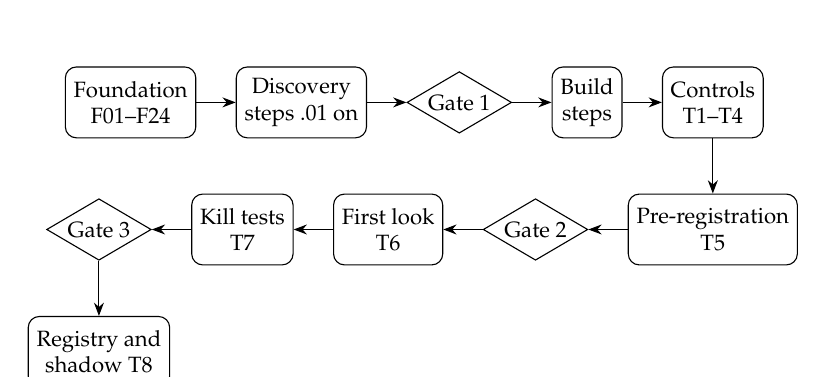
\begin{tikzpicture}[node distance=7mm and 5mm,
  box/.style={draw, rounded corners, align=center, font=\footnotesize, minimum height=9mm, inner sep=3pt},
  gate/.style={draw, diamond, aspect=1.7, align=center, font=\footnotesize, inner sep=1pt},
  >=Stealth]
\node[box] (F) {Foundation\\F01--F24};
\node[box, right=of F] (D) {Discovery\\steps .01 on};
\node[gate, right=of D] (G1) {Gate 1};
\node[box, right=of G1] (B) {Build\\steps};
\node[box, right=of B] (C) {Controls\\T1--T4};
\node[box, below=of C] (P) {Pre-registration\\T5};
\node[gate, left=of P] (G2) {Gate 2};
\node[box, left=of G2] (L) {First look\\T6};
\node[box, left=of L] (K) {Kill tests\\T7};
\node[gate, left=of K] (G3) {Gate 3};
\node[box, below=of G3] (R) {Registry and\\shadow T8};
\draw[->] (F) -- (D);
\draw[->] (D) -- (G1);
\draw[->] (G1) -- (B);
\draw[->] (B) -- (C);
\draw[->] (C) -- (P);
\draw[->] (P) -- (G2);
\draw[->] (G2) -- (L);
\draw[->] (L) -- (K);
\draw[->] (K) -- (G3);
\draw[->] (G3) -- (R);
\end{tikzpicture}
\end{center}
Nothing touches the target before Gate~2, and nothing reaches a quote before Gate~3.

\section{Shared foundation: F01 to F24}
\label{sec:foundation}
Twenty-four steps, run once, before any signal ladder. F01 to F04 are discovery. F05 to F15 build the panels. F16 to F24 build the test rig.

\begin{ladder}[label=\textbf{F\twodigit*}]
\item \stepname{Lake inventory, read-only} List every schema and table with row counts, date ranges, update cadence and owner. \Out \code{foundation/inventory.md}. \Pass a human marks which tables are the tape, security master, quotes, RFQ log and holdings.
\item \stepname{Tape data dictionary} Document every tape field, type, null rate and enumeration. Locate: reporting side, contra-party type, capacity, size and cap flag, ATS flag, portfolio-trade flag, special-price and when-issued flags, cancel and correction indicators, execution and dissemination timestamps. \Out \code{foundation/tape_dictionary.md}. \Pass each concept maps to a field or is reported missing.
\item \stepname{Security master audit} Check the identifier map, issuer hierarchy to ultimate parent and listed equity, coupon, maturity, call schedule, seniority, 144A flag, amount-outstanding history and rating history with announcement times. \Out \code{foundation/secmaster_audit.md}. \Pass 99\% of index-eligible bonds resolve to an issuer, and rating and amount histories are point-in-time.
\item \stepname{Clocks and calendar} Build the business-day calendar, fix the time zone, and write one \code{knowledge_time} rule per dataset. \Out \code{foundation/clocks.yaml}. \Pass every dataset in F01 has a rule, with human sign-off.
\item \stepname{Tape cleaning} Apply cancel, correction and reversal logic. Remove when-issued, special-price and non-standard-settlement prints. De-duplicate inter-dealer double reports. Keep two views: \code{tape_as_seen}, where a correction applies only from its own knowledge time, and \code{tape_clean}. Features read \code{tape_as_seen}; targets read \code{tape_clean}. \Pass the ledger explains every dropped row class, and pilot bond-days reconcile by hand.
\item \stepname{Trade classification} Label customer buy, customer sell and inter-dealer. Bucket size: under 100k, 100k to 1mm, 1mm to cap, capped. Flag agency prints. Flag matched pairs: a customer trade with an offsetting trade of equal par in the same CUSIP within 15 minutes. \Out \code{foundation/trades_classified.parquet}. \Pass matched share is stable month to month, and 30 sampled pairs are verified by eye.
\item \stepname{Capped-size model} Fit $\E[\text{size}\mid\text{capped}]$ by rating class, issue size and year, using only uncapped history already public at $t$. \Out \code{size_hat}. \Pass calibration within 10\% by bucket on held-out quarters.
\item \stepname{Half-spread model} Estimate \code{h_hat} by bond, size bucket and month as half the same-day gap between customer-buy and customer-sell VWAPs, and from matched round trips. \Out \code{foundation/h_hat.parquet}. \Pass monotone in size bucket, coverage reported, fallback hierarchy documented.
\item \stepname{Mid proxy} Build daily \code{mid} by hierarchy: inter-dealer VWAP, else average of customer-buy and customer-sell VWAPs, else side-adjusted price. Exclude trades under \$100k and down-weight portfolio-trade prints. Stamp \code{mid_source} and \code{staleness_days}. Build \code{mid_quote} in parallel if a composite feed exists. \Pass where all sources exist, median disagreement is inside \code{h_hat}.
\item \stepname{Rates hedge} Compute Treasury key-rate returns, analytical key-rate durations, and empirical duration by spread bucket at a 1-day horizon fitted to $t-1$. \Out credit excess returns \code{r_cx} on both mids. \Pass post-hedge correlation with the 10-year Treasury return is near zero in IG and reported for HY.
\item \stepname{Residual returns, forward and trailing} Regress credit excess returns cross-sectionally on DTS, sector-by-rating, maturity bucket and liquidity bucket. The target is $y(i,t,h)=\rres_i(t+1,t+1+h)$ for $h$ of 5 and 10, written to the target store with drop-out flags. The same code writes the trailing panel $\rres_i(t-k,t)$ for $k$ of 1, 5, 10 and 21 to the feature store, because several signals use past residual returns. \Pass zero cross-sectional mean by bucket, and one code path for both panels.
\item \stepname{Tradable residual target} Fit rolling betas to CDX IG and HY, LQD and HYG, and Treasury futures to $t-1$. Add a hedge-cost series and a basis-volatility series. Target store. \Pass every hedge series has a knowledge time and betas are stable.
\item \stepname{Fill and RFQ markout table} Behind Gate~0. From the desk RFQ log take wins with fill price and cover price, and lost RFQs matched to the TRACE winning print. Compute mid at fill time and at $+5$ and $+10$ days. Target store. \Pass at least 98\% of desk wins match the desk's own TRACE reports.
\item \stepname{Cost model} Implement $c_i(q)$ of equation~\eqref{eq:cost} with one column per term. \Pass three hand-computed cases match.
\item \stepname{Universe and liquidity buckets} Apply a point-in-time index-style filter: at least \$250mm outstanding, non-convertible, non-defaulted, over one year to maturity, fixed coupon. Assign liquidity deciles from trailing 60-day volume and trade-day count. \Pass monthly universe count plotted, and no future data in any assignment.
\item \stepname{Evaluation harness} Input a signal panel and a target name. Output IC by horizon, bucketed mean markout with Hansen--Hodrick errors, a non-overlapping block version, a decay curve from 1 to 15 days, the frontier $\mathrm{IC}\,\sigma/c$ by liquidity decile, and turnover. \Pass deterministic, with unit tests.
\item \stepname{Synthetic tape generator} Simulate bonds with a latent mid, bid-ask bounce, sparse trading, capped sizes, and a switchable planted effect with type, size and half-life. \Pass with the effect off, mean IC over 200 seeds is within 2 standard errors of zero, and with it on the effect is recovered within 25\%.
\item \stepname{Leakage audit tool} Assert every feature input has \code{knowledge_time} at or before signal time. Scan code lineage for any join of a signal to a return that ends after the signal's stamp, outside F16. Add a future-shift test: shift the signal forward $k$ days and flag any IC jump. Add as-of join unit tests. \Pass the tool catches three deliberately planted leaks.
\item \stepname{Pre-registration freezer} Template: hypothesis, sign, horizons, universe, buckets, parameters, statistics to report, kill thresholds. Freezing writes a hash to an append-only log. \Pass the harness refuses to run without a matching hash.
\item \stepname{Kill-test runner} Implement the five kill tests as functions that return pass or fail with values. \Pass runs end to end on a synthetic signal.
\item \stepname{Signal registry} Contract: \code{signal_id, bond, knowledge_time, value, version}. Fit an isotonic map from value to bp by liquidity bucket and horizon, to $t-1$. \Pass schema test passes and the map is monotone.
\item \stepname{Gate calibration} Implement the Learn-then-Test threshold on counterfactual fills rebuilt from cover and winning prices, with CLT $p$-values on block means, blocks of at least $2h$ days, plus the rolling update. \Pass on synthetic data, realised risk is below $\alpha$ in at least $1-\delta$ of 500 replications.
\item \stepname{Shadow logger and monitors} Log what the skew would have been per RFQ, changing no quote. Monitor signal decay, input drift, realised against predicted markout, and the gate loss series. \Pass code review confirms no write path to the quoting system.
\item \stepname{Run manifest and CI} Every run writes a manifest: code commit, config hash, input versions, ledger. CI runs unit tests and both synthetic controls on every change. \Pass a clean clone reproduces a pilot artifact exactly.
\end{ladder}

\section{Standard tail: T1 to T8}
\label{sec:tail}
Every ladder ends with the same eight steps. Each signal section supplies the parameters: toy case, planted effect, negative control and exposed kill tests.

\begin{ladder}[label=\textbf{T\arabic*}]
\item \stepname{Toy cases} Code the section's hand-computed toy case as a unit test. Add the edge cases that apply: a bond with no prints in the window, and a capped print. \Pass all values match.
\item \stepname{Positive control} First extend the F17 generator with the section's inputs, such as RFQ arrivals, equity returns or baskets, and review that extension like signal code. Then run the signal code unchanged on the synthetic data with the section's planted effect. \Pass correct sign, magnitude within 25\%.
\item \stepname{Negative control} Run the section's placebo. \Pass IC inside the noise band from 200 seeds.
\item \stepname{Leakage audit} Run the F18 knowledge-time assertions and lineage scan on the real signal panel, and the future-shift test on synthetic data only. \Pass zero violations. The real-data future-shift check waits for T6, because it needs the target.
\item \stepname{Pre-registration} Fill the F19 template with the section's hypothesis, sign, horizons, parameters and thresholds, then freeze it. Gate~2 follows.
\item \stepname{First look} Run F16 on the statistical residual, mid to mid, at 5 and 10 days. Pilot slice first, then full history. Evaluate only on dates after every fitting sample used in the build steps. Report only pre-registered statistics plus the future-shift check. \Pass report complete and no parameter changed.
\item \stepname{Kill tests} Run F20 and output the five-row verdict table. One fail demotes the signal to an input. Two remove it. Gate~3 follows.
\item \stepname{Registry and shadow} Register per F21. Write a one-page signal card: definition, data, parameters, verdict, failure modes. Enable F23 shadow logging for 60 business days. \Pass predicted against realised markout reported weekly, and no quote changed.
\end{ladder}

\section{Gates}
\begin{center}
\begin{tabularx}{\textwidth}{@{}l l l X@{}}
\toprule
Gate & When & Signs & Checks \\
\midrule
Gate 0 & Before F13, A3.01 and B4.01 & Compliance & RFQ data use is permitted, and loan data is public-side \\
Gate 1 & After the discovery steps & Desk quant & Field semantics, sign conventions and coverage \\
Gate 2 & After T5 & Head of research & Hypothesis, sign and thresholds are frozen \\
Gate 3 & After T7 & Head of desk & Verdict, role, and shadow-only status \\
\bottomrule
\end{tabularx}
\end{center}

\section{Build order}
Six waves. Each wave reuses exports from the one before.
\begin{enumerate}[itemsep=2pt]
\item \textbf{Foundation.} F01 to F24. F13 waits for Gate~0.
\item \textbf{Tape only.} A5, then A1, A2, A4. A5 goes first because it exports the veto the others consume. A1 exports the flow panel $I_{i,t}$ used by C1 and D2.
\item \textbf{Calendars and mechanics.} D2, D3, C3, D4, D1.
\item \textbf{Cross-market.} B1, B5, B2, E3, B3. B1 exports the wealth-transfer flag. E3 exports the second veto. Then re-run A1.08 so its veto join picks up B1, B5 and E3.
\item \textbf{Holdings and ETF.} E2, E1, then C1 and C2. Re-run A4 once E2 exports basket membership.
\item \textbf{Gated data.} A3 after Gate~0 and F13. B4 after Gate~0.
\end{enumerate}
\section{Ladders for family A: liquidity provision and dealer balance sheet}
\label{sec:laddersA}
Read the operating rules and finish the shared foundation first. Each ladder lists its dependencies, its build steps, and the parameters for the standard tail T1 to T8.

\subsection{A1. Inventory-conditioned reversal}
\emph{Needs F05 to F09, F11 and F15. Exports the flow panel $I_{i,t}$ to C1 and D2. Nine build steps, then T1 to T8.}
\begin{ladder}[label=\textbf{A1.\twodigit*}]
\item \stepname{Side-convention discovery} For one liquid bond-day, print 20 classified rows and state in words who bought from whom. \Out \code{A1/discovery.md}. \Pass Gate~1 confirms that a plus sign means a dealer bought from a customer.
\item \stepname{Signed dealer flow} Set $q=+\mathrm{par}$ when a dealer buys from a customer, $-\mathrm{par}$ when it sells to one, and 0 for inter-dealer. Drop matched pairs and agency prints. \Out \code{A1/flow_trades.parquet}. \Pass dropped rows reconcile to the F06 flags.
\item \stepname{Capped sizes, two ways} Build \code{q_floor} from the cap itself and \code{q_hat} from F07. Keep both. \Pass \code{q_hat >= q_floor} on every capped row.
\item \stepname{Daily and 5-day flow} Sum $q$ by bond and day, roll 5 business days, and divide by point-in-time amount outstanding to get $I_{i,t}$. \Pass list the 20 largest $|I|$, and send any above 20\% of outstanding to manual review.
\item \stepname{Past residual return} Read $\rres_i(t-5,t)$ from the F11 trailing panel. Require two mids in the window, else null. It is a trailing return, which rule~6 allows. \Pass null rate reported by liquidity decile.
\item \stepname{Opposite-sign gate and rank} $S=-\rres\cdot\ind{\rres\,I<0}\cdot\mathrm{rank}(|I|)$, ranked within liquidity bucket on 0 to 1. Build \code{S_floor} and \code{S_hat}. \Pass $S$ is zero whenever price and inventory moved the same way.
\item \stepname{Conditioning flags} Add an HY flag, a CDS-exists flag, and a stress flag for VIX above its 80th percentile. \Pass all point-in-time.
\item \stepname{Veto join} As-of join the A5, B1, B5 and E3 veto flags and set $S=0$ under any of them, except that the E3 veto zeroes only positive values. A producer that does not exist yet defaults to no veto and is logged. \Pass veto coverage reported.
\item \stepname{Time stamp} Stamp \code{knowledge_time} at 17:30 ET using prints disseminated by 17:15. \Pass no input is later than the stamp.
\end{ladder}
\textbf{Tail parameters.} Toy case: $\rres=-40\bp$, $I=+2\%$, rank 0.9 gives $S=+36$; the same return with $I=-2\%$ gives 0. Planted effect: 30\% of a flow-driven concession reverts over 5 days. Negative control: shuffle $I$ across bonds within day and bucket. Exposed kill tests: mid to mid and post-2020. Pre-registered interactions: stronger in HY, without CDS, and in stress.

\subsection{A2. Post-block offload path}
\emph{Needs F05 to F09 and F11. Consumes the A5 veto. Nine build steps, then T1 to T8.}
\begin{ladder}[label=\textbf{A2.\twodigit*}]
\item \stepname{Capped-print census} Count capped prints by month, rating class and side, and the share that are principal with no matched offset. \Out \code{A2/discovery.md}. \Pass the cap flag and the size-equals-cap rule agree on 99\% of rows.
\item \stepname{Event table} One row per capped, principal, unmatched customer trade: bond, dissemination time, side, price and \code{mid_pre}. \code{mid_pre} is the prior business day's F09 mid, at most 3 business days old, so it cannot contain the block print. \Pass events with no valid \code{mid_pre} are dropped and counted.
\item \stepname{Concession} $\kappa=(P^{\mathrm{block}}-\text{\code{mid_pre}})/\text{\code{mid_pre}}$ in bp, net of the same-day bucket mean return, so a market move is not read as a concession. \Pass median $\kappa$ is negative for customer sells and positive for customer buys.
\item \stepname{Episode merge} Merge same-side blocks in one bond within 10 business days into one episode, with summed \code{size_hat} and volume-weighted $\kappa$. \Pass no bond has overlapping episodes.
\item \stepname{Parent-order tracker} Track later same-side prints of \$1mm or more. Set \code{flow_stopped} on the first day that follows two clear business days. \Pass 10 episodes hand-checked.
\item \stepname{Size scale} $g=\min(1,\ \text{\code{size_hat}}/\ADV^{20})$. \Pass $g$ lies in 0 to 1.
\item \stepname{Signal} $S=-\kappa\,g$ from the \code{flow_stopped} day to day 10 of the episode. Zero before, after, and under veto. \Pass a state-machine unit test over a 15-day synthetic episode.
\item \stepname{Resale feature} Flag dealer-to-customer sells after a customer-sell block at prices above the block price (mirror for customer-buy blocks). Optional interaction. \Pass point-in-time.
\item \stepname{Pre-event view} Plot mid paths from day $-5$ to day 0 only. The forward path waits for T6. \Pass no forward data read.
\end{ladder}
\textbf{Tail parameters.} Toy case: a customer sell at 98.50 against \code{mid_pre} 99.00 and a flat bucket gives $\kappa=-50.5\bp$; with $g=0.6$, $S=+30.3$ from the \code{flow_stopped} day and 0 before. Planted effect: 40\% of $\kappa$ recovered by day 5. Negative control: placebo events on matched non-event bond-days. Exposed kill tests: mid to mid and fill-conditional.

\subsection{A3. Latent RFQ imbalance}
\emph{Needs F03, F09, F13 and F15. Starts at Gate~0. Eleven build steps, then T1 to T8.}
\begin{ladder}[label=\textbf{A3.\twodigit*}]
\item \stepname{Gate 0: permitted use} A human confirms in writing that inquiry data may inform pricing research under platform rules and internal barriers. \Out \code{A3/gate0.md}. \Pass signed. No query runs before this.
\item \stepname{RFQ log discovery} Document platforms, coverage dates, daily counts and fields: timestamp, bond, client side, size, dealers in competition, desk response, outcome, cover price, hashed client id and tier. Check clock sync against the tape. \Out \code{A3/discovery.md}. \Pass Gate~1 confirms outcome codes and side semantics.
\item \stepname{Canonical table} Normalise to the client view: a client buy is a request at the desk's offer. Hash any raw client id. \Out \code{A3/rfq.parquet}. \Pass no raw client identifier in any artifact.
\item \stepname{Outcome matching} Match each RFQ to tape prints in the same CUSIP and side, size equal or capped, from 1 minute before to 30 minutes after the RFQ closes. Label \code{traded} with the winning price, or \code{did_not_trade}. \Pass at least 98\% of the desk's own wins match.
\item \stepname{Repeat-inquiry chains} Link inquiries sharing hashed client, bond, side and similar size within 5 business days. Count failed attempts per chain. \Pass 20 chains hand-checked.
\item \stepname{Weighted intensities} Per bond and side, keep exponentially weighted counts $\nu^{+}$ and $\nu^{-}$ with a 2-day half-life. Weight a \code{did_not_trade} inquiry 2 and a filled one 1. Add a size-weighted variant. An outcome label is known only 30 minutes after the inquiry closes, so stamp it then. \Pass counts use only inquiries and labels known strictly before the stamp.
\item \stepname{Imbalance and shrinkage} $\Imb_i=(\nu^{+}-\nu^{-})/(\nu^{+}+\nu^{-})$ and $n_i=\nu^{+}+\nu^{-}$. Shrink to the issuer, then to the sector-rating-maturity cluster: $\Imb^{\mathrm{post}}=(n_i\,\Imb_i+\tau\,\Imb^{\mathrm{cl}})/(n_i+\tau)$. Fit $\tau$ by method of moments on the first third of the sample only. \Pass $\Imb^{\mathrm{post}}$ lies between $\Imb_i$ and $\Imb^{\mathrm{cl}}$.
\item \stepname{Market-share diagnostic} Compute the desk's share of tape customer volume by bucket and month, and attach it as a reliability weight. \Pass reported, because the review left this as its open question.
\item \stepname{Kernel features} Build $\Imb^{\mathrm{post}}$ at half-lives of 1, 3 and 10 days, so pressure and later reversal can load separately. \Pass three columns with one stamp.
\item \stepname{Self-exclusion} When scoring an incoming RFQ, exclude that RFQ and everything after it from the imbalance. \Pass an assertion on strict timestamp order.
\item \stepname{Two targets} Register the signal against both the composite-mid change and the F13 fill-conditional markout. \Pass both appear in the pre-registration.
\end{ladder}
\textbf{Tail parameters.} Toy case: weighted counts of 6 buys and 2 sells give $\Imb_i=0.5$; with $n_i=8$, $\tau=8$ and $\Imb^{\mathrm{cl}}=0.1$, $\Imb^{\mathrm{post}}=(8\times0.5+8\times0.1)/16=0.30$. Planted effect: RFQ arrivals from a two-state Markov-modulated Poisson process whose hidden state drives mid drift. Negative control: shuffle RFQ sides within bond-day. Exposed kill tests: fill-conditional, plus IC reported as a function of desk market share.

\subsection{A4. Portfolio-trade leg pressure}
\emph{Needs F05, F06, F09 and F15. Uses ETF ownership now and E2 basket membership later. Nine build steps, then T1 to T8.}
\begin{ladder}[label=\textbf{A4.\twodigit*}]
\item \stepname{Flag discovery} Report the portfolio-trade flag's field name, first populated date and monthly share of volume. Sample 50 flagged prints. \Out \code{A4/discovery.md}. \Pass flagged prints arrive in same-second clusters of many CUSIPs.
\item \stepname{Basket reconstruction} Cluster flagged prints by execution second, side and reporting pattern into \code{basket_id}. Record line count, par and net customer direction. \Pass 20 baskets hand-checked, and singletons counted as unresolved.
\item \stepname{Line deviation} $\mathrm{dev}=(P^{\mathrm{PT}}-\Pm)/\Pm$ in bp, against an F09 mid built without portfolio-trade prints. \Pass mean dev within a basket is negative for customer-sell baskets and positive for customer-buy baskets, with dispersion reported.
\item \stepname{Dealer PT position} Per bond and day, sum par dealers bought from customers in baskets, minus par sold. \Pass signs reconcile to the A1 convention.
\item \stepname{Outlet score} Build \code{outlet} on 0 to 1 from point-in-time ETF ownership share, and from creation-basket membership once E2 exists. \Pass knowledge times respect holdings lags.
\item \stepname{Resale detection} After a basket, flag dealer sells in that bond within 5 days and set \code{resale_started}. \Pass 10 cases hand-checked.
\item \stepname{Signal} $S=(Q^{\mathrm{PT}}/\ADV^{20})\,(1-\text{\code{outlet}})$, active from \code{resale_started} or day 2, whichever comes first, to day 10. \Pass state-machine unit test.
\item \stepname{Hygiene export} Export the flag to F09 so mids down-weight these prints. \Pass a regression test shows F09 changes only on bond-days with flagged prints.
\item \stepname{Secondary hypothesis} Pre-register the outlet interaction separately, because the literature disagrees on it. \Pass two hypotheses in the template.
\end{ladder}
\textbf{Tail parameters.} Toy case: dealers buy \$4mm in baskets, $\ADV=\$8$mm and \code{outlet} $=0.4$, so $S=0.5\times0.6=0.30$. Planted effect: 20 bp of offload pressure that reverts by day 8. Negative control: same-issuer bonds that were not in the basket. Exposed kill tests: mid to mid and term structure.

\subsection{A5. Informed-flow continuation}
\emph{Needs F05, F06, F08, F09 and F15. Exports \code{veto_L}, so build it first in wave 2. Eight build steps, then T1 to T8.}
\begin{ladder}[label=\textbf{A5.\twodigit*}]
\item \stepname{Matched-pair audit} Report the time-gap distribution of F06 matched pairs and the matched share by year and size bucket. \Out \code{A5/discovery.md}. \Pass no unexplained structural break, then Gate~1.
\item \stepname{Signed matched flow} Sign each pair by its initiating side, buy as plus. With one customer leg, use that customer's side. With two customer legs, the pair is sell-initiated if its VWAP is below the prior F09 mid, buy-initiated if above, and null within a quarter of \code{h_hat}. Keep pairs of \$1mm or more, capped prints included. $F^{m}_i(t-3,t)$ is that flow over ADV. \Pass inter-dealer-only chains are excluded, and the null share is reported.
\item \stepname{Abnormal volume} On days with trades, flag log volume more than 2 standard deviations above its mean over the last 60 trade days. \Pass flag rate between 2\% and 8\% of trade days.
\item \stepname{Signal} $S=z(F^{m})\cdot\text{\code{abnormal}}$, $z$-scored cross-sectionally within liquidity bucket. \Pass zero on normal-volume days.
\item \stepname{Issuer propagation} Take the value from the issuer's most active bond by trailing 60-day volume. Apply half of it to the issuer's other bonds. \Pass the most-active ranking is point-in-time.
\item \stepname{Earnings hook} Expose $F^{m}$ by issuer and day so that B5.07 can build $S^{\mathrm{pre}}$. No earnings data is read here. \Pass schema test.
\item \stepname{Veto export} Set \code{veto_L = 1} for the issuer for 5 business days when $|S|$ exceeds 1.5. \Out \code{A5/veto.parquet} for A1, A2, C1, D2, E1 and E2. \Pass schema test and coverage report.
\item \stepname{Mirror check} Run the same formula on unmatched principal flow. It should revert where matched flow persists, which makes it the discriminating control. \Pass built and ready for T3.
\end{ladder}
\textbf{Tail parameters.} Toy case: matched customer buys of \$6mm against $\ADV=\$3$mm give $F^{m}=2.0$; on an abnormal day $S$ equals its $z$-score, and the same flow unmatched gives 0 here and feeds A1. Planted effect: a permanent 25 bp shift after matched flow, with no reversal. Negative control: the A5.08 mirror. Exposed kill tests: mid to mid and fill-conditional.

% =====================================================================
\section{Ladders for family B: cross-market information diffusion}
\label{sec:laddersB}

\subsection{B1. Unabsorbed equity information}
\emph{Needs F03, F09, F10, F11 and F15. Exports \code{wt_flag}. Ten build steps, then T1 to T8.}
\begin{ladder}[label=\textbf{B1.\twodigit*}]
\item \stepname{Issuer-equity map discovery} Report the share of bonds whose ultimate parent has listed equity, by rating class. List private issuers as excluded. Check corporate-action handling and the equity price source. \Out \code{B1/discovery.md}. \Pass Gate~1 reviews the mapping of the 50 largest HY issuers by hand.
\item \stepname{Clock alignment} Equity closes at 16:00 ET and the bond mid is stamped later. Fix the rule: the equity return through the close of day $t$ pairs with bond mids through day $t$. \Pass written into \code{clocks.yaml}.
\item \stepname{Equity idiosyncratic return} Take the residual of daily stock return on market and sector ETF returns, with 252-day rolling betas fitted to $t-1$. \Pass residual correlation with the market is near zero.
\item \stepname{Maturity rank} Rank each bond's maturity within its issuer's outstanding bonds, point-in-time, scaled 0 to 1. \Pass single-bond issuers get 0.5.
\item \stepname{Hedge-ratio panel} Regress 5-day trailing bond residuals from F11 on 5-day equity idiosyncratic returns within rating, leverage-tercile and maturity-rank buckets. Use an expanding window to $t-1$, shrink to the bucket mean, floor at 0. \Out \code{beta_E(i,t)}. \Pass $\beta^{E}$ rises with maturity rank and falls with rating quality.
\item \stepname{Unabsorbed term} $U=\beta^{E}\sum_{u=t-4}^{t}r^{E,\mathrm{idio}}_u-\rres(t-5,t)$ on mids, so both terms span the same five trading days. Flag rows whose bond mid is over 3 days stale. \Pass stale share reported by liquidity decile.
\item \stepname{Wealth-transfer override} Set \code{wt_flag} for 10 days on tags for M\&A, LBO, large buyback, special dividend or activist filing, each with its knowledge time. Also set it when equity is up, implied vol is up and the bond is down beyond pre-registered thresholds. Under the flag $U=0$. \Out \code{B1/wt_flag.parquet}. \Pass 20 historical LBO cases trigger the flag.
\item \stepname{Earnings hand-off} Zero $U$ on days 0 to $+2$ of an earnings announcement, and drop those days from both sums in any later window that spans them. B5 owns the earnings reaction. \Pass a synthetic earnings jump leaves the signal unchanged outside B5.
\item \stepname{Tail definition} Define the standalone test set: $|z(U)|$ above 2.5, HY and crossover names, the issuer's most liquid bond. \Pass tail events per month reported.
\item \stepname{Taker backtest stub} Prepare entry at mid plus \code{h_hat} and exit at mid minus \code{h_hat}, under the F16 fill-realism rule. It runs only in T6. \Pass code reviewed, not executed.
\end{ladder}
\textbf{Tail parameters.} Toy case: $\beta^{E}=0.10$ and a 5-day equity idiosyncratic sum of $+8\%$ imply $+80\bp$; the bond realised $+20\bp$, so $U=+60\bp$, and under \code{wt_flag} it is 0. Planted effect: the bond absorbs half of an equity shock on day 0 and the rest over 3 days. Negative control: re-pair issuers and equities at random within sector. Exposed kill tests: mid to mid with the one-day skip, and term structure.

\subsection{B2. Option-implied volatility innovation}
\emph{Needs F03, F15 and B1.03. Eight build steps, then T1 to T8.}
\begin{ladder}[label=\textbf{B2.\twodigit*}]
\item \stepname{Options data discovery} Document the vendor surface: delta and tenor grid, timestamp, open-interest and volume fields, and coverage among bond issuers. Fix the knowledge time: an end-of-day surface is known the next business day. \Out \code{B2/discovery.md}. \Pass Gate~1.
\item \stepname{IV level} Average 50-delta call and put IV at 30, 60 and 91 days, with a minimum open-interest filter. \Pass coverage by rating class reported.
\item \stepname{IV changes} Take log changes over 5 and 21 trading days, winsorised at 1\%. \Pass both columns present.
\item \stepname{Earnings mask} Drop any window that spans an earnings date, because IV collapses mechanically after the announcement. \Pass masked share reported.
\item \stepname{Orthogonalise} Each day, regress the IV change cross-sectionally on the issuer's equity return over the same window and on $\beta\,\Delta\mathrm{VIX}$. Keep the residual \code{dIV_perp}. \Pass the residual is uncorrelated with both regressors.
\item \stepname{Signal} $S=-z(\text{\code{dIV_perp}})$ within rating bucket, applied to all the issuer's bonds. \Pass the issuer-level value is identical across its bonds.
\item \stepname{Overlap check with B1} Report the correlation between $S$ and B1's $U$. \Pass below 0.3, else revisit B2.05.
\item \stepname{Horizon variants} Register the 5-day and 21-day change versions as separate signals. \Pass both named in the pre-registration.
\end{ladder}
\textbf{Tail parameters.} Toy case: a raw change of $+5$ vol points, of which the equity drop explains $+3$, leaves \code{dIV_perp} $=+2$ and a negative $S$. Planted effect: 10 bp of spread widening over 10 days per residual vol point. Negative control: the IV change of a random same-sector issuer. Exposed kill test: term structure, because the published evidence is monthly.

\subsection{B3. Idiosyncratic basis innovation}
\emph{Needs F03, F08, F09, F10 and F15. Ten build steps, then T1 to T8.}
\begin{ladder}[label=\textbf{B3.\twodigit*}]
\item \stepname{CDS data discovery} Document tenors, document clause, currency, contributor depth and timestamps of the single-name composites. Map reference entities to the issuer hierarchy. \Out \code{B3/discovery.md}. \Pass Gate~1 reviews the entity map for index constituents.
\item \stepname{Liquidity screen} Keep names with at least 3 contributors at 5 years and a spread that changed on at least 3 of the last 5 days. \Pass screened universe size reported by month.
\item \stepname{Bond spread measure} Compute $Z$-spread from the F09 mid. Exclude bonds priced more than 10 points from par, and callable bonds trading to call. \Pass $Z$-spreads reconcile to a vendor value on a 100-bond sample.
\item \stepname{Maturity matching} Interpolate the CDS curve log-linearly to each bond's maturity. \Pass no extrapolation beyond the first or last tenor.
\item \stepname{Raw basis} $\mathrm{basis}=\mathrm{CDS}_{\mathrm{interp}}-Z$ in bp. \Pass distribution by rating plotted.
\item \stepname{Friction regression} Each day, regress the basis cross-sectionally on \code{h_hat}, rating dummies, dollar price, contributor depth and amount outstanding. Keep \code{resid_basis}. \Pass coefficients are stable through time.
\item \stepname{Index component} Estimate each issuer's beta to the index-level basis on a rolling window to $t-1$, and remove it. \Pass the residual is uncorrelated with the index basis.
\item \stepname{Innovation term} $\mathrm{innov}=-\bigl(\SD\,\Delta\mathrm{CDS}(t-5,t)+\rcx(t-5,t)\bigr)$, the CDS-implied bond move not yet realised, with $\rcx$ the F10 credit excess return. \Pass the toy case below.
\item \stepname{Signal} $S=-z(\text{\code{resid_basis}})+z(\mathrm{innov})$, with both components also registered separately. \Pass signs match Part~II.
\item \stepname{Package variant} Build the P\&L of the bond plus a DV01-matched CDS, net of CDS bid-ask, as a second evaluation series. Runs only in T6. \Pass code reviewed, not executed.
\end{ladder}
\textbf{Tail parameters.} Toy case: $\SD=5$, $\Delta\mathrm{CDS}=+10\bp$ and $\rcx=-10\bp$ give $\mathrm{innov}=-(50-10)=-40\bp$, so the bond is expected to fall further. Planted effect: the bond closes half of the residual basis over 10 days. Negative control: permute CDS curves across issuers within rating bucket. Exposed kill test: term structure, because the published result is at 20 days.

\subsection{B4. Loan-to-bond lead}
\emph{Starts at Gate~0. Needs F03, F09, F11 and F15. Exploratory. Nine build steps, then T1 to T8.}
\begin{ladder}[label=\textbf{B4.\twodigit*}]
\item \stepname{Gate 0: public-side confirmation} Compliance confirms in writing that the loan price feed and the research environment are public-side. \Out \code{B4/gate0.md}. \Pass signed. No loan data is queried before this.
\item \stepname{Loan data discovery} Document facility identifiers, bid and ask marks, quote depth, facility type, maturity and borrower name. \Out \code{B4/discovery.md}. \Pass Gate~1.
\item \stepname{Borrower-to-issuer map} Map loan borrowers to bond issuers through the hierarchy. Loans often sit at an operating company and bonds at a holding company. \Pass the 100 largest HY issuers reviewed by hand.
\item \stepname{Coverage} Count issuers with an institutional term loan of at least \$500mm and index-eligible unsecured bonds, by month. \Pass at least 100 issuers on average, else stop and report.
\item \stepname{Loan return} Take the 5-day change in the mid mark. Drop marks unchanged for 5 days or with depth below 2. \Pass stale share reported.
\item \stepname{Knowledge lag} End-of-day marks are known the next morning, so lag them one business day. \Pass an assertion inside the join.
\item \stepname{Theta by bucket} Regress contemporaneous bond residual return on loan return, by loan-price bucket (97 and above, 90 to 97, below 90) and bond seniority, expanding to $t-1$. \Pass $\theta$ rises as the loan price falls.
\item \stepname{Signal} $S=\theta_b\,r^{\mathrm{loan}}(t-5,t)-\rres(t-5,t)$. \Pass the toy case below.
\item \stepname{Exploratory status} Mark the pre-registration exploratory and raise the $t$-statistic threshold to 3.5, because no published bond-return test exists. \Pass threshold in the template.
\end{ladder}
\textbf{Tail parameters.} Toy case: $\theta=1.5$ and a loan move of $-100\bp$ imply $-150\bp$; the bond realised $-50\bp$, so $S=-100\bp$. Planted effect: the bond follows the loan with a 3-day lag. Negative control: loans of a random same-sector borrower. Exposed kill test: mid to mid, because loan marks are quotes and bond mids are partly trades, and that asymmetry in staleness can fake a lead.

\subsection{B5. Bond PEAD with pre-announcement flow}
\emph{Needs F03, F09, F11, F15 and the A5.06 hook. Ten build steps, then T1 to T8.}
\begin{ladder}[label=\textbf{B5.\twodigit*}]
\item \stepname{Earnings data discovery} Document announcement dates and times, whether each date was pre-announced, consensus estimates with their own timestamps, and the issuer mapping. Private issuers with public debt have no consensus and are excluded. \Out \code{B5/discovery.md}. \Pass Gate~1.
\item \stepname{Day-zero rule} An announcement after the close belongs to the next business day. \Pass unit test on before-open, intraday and after-close cases.
\item \stepname{SUE} Actual minus the consensus mean as of day $-1$, scaled by the share price at day $-1$, winsorised at 1\%, with a dispersion-scaled variant. \Pass the consensus snapshot has a knowledge time before day 0.
\item \stepname{Equity CAR} Market-adjusted return over days 0 to $+2$. \Pass aligned to the day-zero rule.
\item \stepname{Bond announcement control} Trailing bond residual over days $-1$ to $+2$, kept as a control and not as a signal. \Pass built from mids.
\item \stepname{Post signal} $S^{\mathrm{post}}=z(\mathrm{SUE})+z(\mathrm{CAR})$, active from day $+2$ for 10 business days, by rating class. \Pass zero outside the window.
\item \stepname{Pre signal} $S^{\mathrm{pre}}$ is built here from the A5.06 hook: signed matched flow in the issuer's most active bond over days $-5$ to $-1$ of the B5.02 calendar. \Pass uses only pre-announcement prints.
\item \stepname{Volume tercile} Tag bonds by trailing 60-day volume tercile, because the literature finds stronger drift in heavily traded bonds. Pre-register this interaction. \Pass the tercile is point-in-time.
\item \stepname{Busy-day control} Count same-day announcers. \Pass column present.
\item \stepname{Taker backtest stub} Entry on day $+2$ at mid plus \code{h_hat}, exit on day $+12$ at mid minus \code{h_hat}, under the F16 fill-realism rule. Runs only in T6. \Pass code reviewed, not executed.
\end{ladder}
\textbf{Tail parameters.} Toy case: results after the close on a Tuesday make Wednesday day 0, and the signal switches on Friday. Planted effect: 15 bp of drift over days $+2$ to $+12$ per unit of $S^{\mathrm{post}}$. Negative control: shift announcement dates by 30 business days. Exposed kill tests: term structure and post-2020.
\section{Ladders for family C: curve and structural relative value}
\label{sec:laddersC}

\subsection{C1. Flow-attributed curve residual}
\emph{Needs the issuer curve model, A1.04, F09 and F15. Nine build steps, then T1 to T8.}
\begin{ladder}[label=\textbf{C1.\twodigit*}]
\item \stepname{Curve model discovery} Find the existing issuer-curve outputs: fitted spread per bond and day, which bonds entered each fit, and knowledge times. \Out \code{C1/discovery.md}. \Pass Gate~1. If no curve model exists, stop, because building one is its own project.
\item \stepname{Fit eligibility} Keep issuers with at least 4 senior unsecured bullet bonds over 1 year. Exclude callables near call and subordinated lines. \Pass eligible issuer count by month.
\item \stepname{Leave-one-out residual} Compute $e_i$ as bond $i$'s spread minus the curve fitted without bond $i$. A self-fitted residual mean-reverts mechanically. \Pass leave-one-out and in-fit residuals differ most for issuers with few bonds.
\item \stepname{Residual change} $\Delta e_i$ over 5 business days in bp. Require mids at both ends, else null. \Pass null rate reported.
\item \stepname{Flow join} As-of join A1's $I_{i,t}$ with the same sign convention. \Pass the convention is asserted in code.
\item \stepname{Pressure coefficient} Regress $\Delta e$ on $I$ by liquidity bucket, expanding to $t-1$, and store $b_t$. \Pass $b>0$ in every bucket, else stop and report.
\item \stepname{Signal} $S=\SD\,(b\,I+\varphi\,e)$ with $\varphi=0.25$, zero under the A5 veto. \Pass the toy case below.
\item \stepname{Half-life} Fit an OU half-life of $e$ per bucket on the first third of the sample. \Pass reported with confidence bands.
\item \stepname{Switch-pair export} Within each issuer, rank bonds by $S$ and export DTS-neutral pairs of cheapest against richest, for list and portfolio-trade line selection. \Pass pair weights are DTS-neutral within 1\%.
\end{ladder}
\textbf{Tail parameters.} Toy case: $\SD=6$, $b\,I=+3\bp$, $\varphi=0.25$ and $e=+8\bp$ give $S=6\times(3+2)=+30\bp$. Planted effect: flow pushes one bond 4 bp off its curve and the gap closes over 8 days. Negative control: the flow of a different bond of the same issuer. Exposed kill tests: mid to mid and fill-conditional.

\subsection{C2. Issuer and supply-chain diffusion}
\emph{Needs F03, F06, F09 and F15. Nine build steps, then T1 to T8.}
\begin{ladder}[label=\textbf{C2.\twodigit*}]
\item \stepname{Link data discovery} Document the issuer hierarchy and the supply-chain source: link start and end dates, revenue share, and the filing date that made each link public. \Out \code{C2/discovery.md}. \Pass Gate~1.
\item \stepname{Leader set} Each day, leaders are bonds with a print of \$1mm or more and a mid built from that day's prints. \Pass leader share of the universe reported.
\item \stepname{Within-issuer adjacency} Weight leader $j$ for follower $i$ by $\exp(-|\mathrm{dur}_i-\mathrm{dur}_j|/2)$ times leader liquidity. Row-normalise with a zero diagonal. \Pass every row sums to 1 or 0.
\item \stepname{Gap since last print} For each follower, accumulate the leaders' weighted residual moves since the follower's own last mid. Call it \code{gap}. A missing print is unobserved, not a zero return. \Pass \code{gap} resets to 0 on the day the follower prints.
\item \stepname{Within-issuer signal} $S^{\mathrm{in}}=\text{\code{gap}}$. \Pass the toy case below.
\item \stepname{Supply-chain adjacency} Customer to supplier at issuer level, weighted by revenue share. Issuer return is the liquidity-weighted mean of its leaders' residual returns. \Pass links use filing knowledge times.
\item \stepname{Supply-chain signal} $S^{\mathrm{sc}}$ from customers' 5-day and 21-day issuer returns, net of the supplier's own return over the same window. \Pass two horizon columns.
\item \stepname{Edge whitelist} Assert the graph holds only same-issuer and supply-chain edges. Generic sector or rating peers are excluded by design. \Pass assertion in code.
\item \stepname{Fair-value export} Send \code{gap} to the F09 mid as a nowcast input, registered as fair value and not as alpha. \Pass registry role field set.
\end{ladder}
\textbf{Tail parameters.} Toy case: a follower last printed 3 days ago and its leaders' weighted residual move since then is $+25\bp$, so $\text{\code{gap}}=S^{\mathrm{in}}=+25\bp$. Planted effect: followers absorb leader moves with a 2-day lag. Negative control: a random graph with the same degree distribution. Exposed kill test: mid to mid. Pre-registered expectation: the within-issuer part mostly vanishes on composite quotes.

\subsection{C3. Quoting-convention pass-through lag}
\emph{Needs F09, F10 and F15. Eight build steps, then T1 to T8.}
\begin{ladder}[label=\textbf{C3.\twodigit*}]
\item \stepname{Convention discovery} Find any field that records whether a bond is quoted on spread or on price, such as dealer runs. If none exists, document the rule-based proxy. \Out \code{C3/discovery.md}. \Pass Gate~1.
\item \stepname{Convention classifier} Point-in-time rule: price-quoted if in an HY index, or priced below 90, or at a spread above 400 bp. Tag the boundary set: bonds within 60 days of an index switch between IG and HY. \Pass the classifier agrees with C3.01 data where that exists.
\item \stepname{Horizon durations} Regress $k$-day mid-to-mid total return on minus the matched key-rate yield change, by spread bucket, rolling 2 years to $t-1$. Use $k=1$, and $k=10$ on non-overlapping windows. \Out $\mathrm{ED}^{(1)}$ and $\mathrm{ED}^{(10)}$ with standard errors. \Pass IG buckets show both near analytical duration.
\item \stepname{Precondition test} Test $\mathrm{ED}^{(10)}=\mathrm{ED}^{(1)}$ per bucket. Where it is not rejected, the signal is off. \Pass a decision table by bucket.
\item \stepname{Signal} $S=(\mathrm{ED}^{(10)}-\mathrm{ED}^{(1)})\,(-\Delta y(t-1,t))$ in bp of price, only when $|\Delta y|$ exceeds 5 bp. \Pass the toy case below.
\item \stepname{Hedge consistency} Record which duration the F10 hedge uses. The forecast is a price move unrelated to Treasury moves inside the target window, so either choice is valid, but the evaluation must state it. \Pass stated in the pre-registration.
\item \stepname{Boundary variant} Register a second signal restricted to the boundary set. \Pass both in the pre-registration.
\item \stepname{Latency note} From the quote logs, read-only, record the time from a 5 bp Treasury move to the desk's HY quote refresh. \Pass reported as context for T8.
\end{ladder}
\textbf{Tail parameters.} Toy case: $\mathrm{ED}^{(10)}=3.0$, $\mathrm{ED}^{(1)}=1.5$ and a 10 bp rally give $S=+15\bp$. Planted effect: price-quoted bonds absorb half of a rates move on day 0 and the rest over 5 days. Negative control: the spread-quoted IG bucket, which should show zero. Exposed kill tests: mid to mid and post-2020.

% =====================================================================
\section{Ladders for family D: event and calendar flows}
\label{sec:laddersD}

\subsection{D1. New-issue concession spillover}
\emph{Needs F03, F09 and F15. Uses the curve model if C1.01 has found one, otherwise spread net of bucket. Nine build steps, then T1 to T8.}
\begin{ladder}[label=\textbf{D1.\twodigit*}]
\item \stepname{Calendar discovery} Document the new-issue feed: announcement time, pricing time, size, tranche maturities, initial talk, guidance, final spread, book size and use of proceeds, with coverage by year. \Out \code{D1/discovery.md}. \Pass Gate~1 confirms announcement times are intraday timestamps, not dates.
\item \stepname{Deal table} One row per deal and tranche, mapped to issuer and sector, with \code{knowledge_time} set to the announcement time. Most deals announce and price the same day, so fix \code{mid_pre} as the prior close and \code{mid_post} as the pricing-day close. \Pass both mids exist, else the deal is dropped and counted.
\item \stepname{Existing-bond set} For each deal, list the issuer's index-eligible bonds outstanding at announcement, with adjacency weight $a_j=\exp(-|T_j-T_{\mathrm{new}}|/3)$. \Pass the new tranches themselves are excluded.
\item \stepname{Widening measure} $w_j$ is the change in bond $j$'s curve residual, or its spread net of its bucket, from \code{mid_pre} to \code{mid_post}. Use composite quotes and inter-dealer prints only. \Pass customer prints are excluded, because underwriter-affiliated dealers may support prices.
\item \stepname{Relative size} Deal size over the issuer's index-eligible debt outstanding. \Pass point-in-time amounts.
\item \stepname{Signal} $S_j=w_j\,\SD_j\,\text{\code{rel_size}}\,a_j$, active from the day after pricing to day 10. \Pass the toy case below.
\item \stepname{Sector variant} The same construction for same-sector, maturity-adjacent bonds of other issuers, scaled by the week's sector supply over sector debt. \Pass the issuer's own bonds are excluded.
\item \stepname{Concession context} Record the new bond's concession: final spread minus the pre-announcement curve at that maturity. Context only. \Pass column present.
\item \stepname{Placebo set} Collect announced deals that were postponed or pulled, if the feed records them. \Pass count reported, which may be zero.
\end{ladder}
\textbf{Tail parameters.} Toy case: an existing 10-year widens 6 bp into pricing, with $\SD=8$, \code{rel_size} $=0.15$ and adjacency 1, so $S=6\times8\times0.15=+7.2\bp$. Planted effect: 37\% of the widening reverts over 10 days, which is a 15-day half-life. Negative control: pseudo-deals on random dates for the same issuer. Exposed kill tests: term structure and post-2020.

\subsection{D2. Index-exit forced flow}
\emph{Needs F03, F09, F15 and A1.04. Ten build steps, then T1 to T8.}
\begin{ladder}[label=\textbf{D2.\twodigit*}]
\item \stepname{Index data discovery} Document which index families have point-in-time constituent history, plus their rule documents, rating rules and lock-out dates. \Out \code{D2/discovery.md}. \Pass Gate~1 confirms which family each rule below refers to.
\item \stepname{Rule engine} As of the lock-out date, project next month-end exits: remaining maturity under 1 year at the rebalance date, or index rating below IG. \Pass precision and recall of at least 98\% against actual historical exits.
\item \stepname{Knowledge time} Stamp each projected exit at the lock-out, which is the third business day before month-end for the ICE family. Other families use their own documented rule. \Pass a rule cited per family.
\item \stepname{Passive ownership} Share of each bond held by ETFs and index funds, point-in-time with filing lags. \Pass coverage reported.
\item \stepname{Event table} Bond, exit type, exit date, knowledge time, passive share, ADV, and for downgrades the equity CAR at the rating date. \Pass one row per bond-exit.
\item \stepname{Information filter} Keep downgrade exits only when the absolute equity CAR over days 0 to $+2$ at the rating date is under 3\%. Keep all maturity exits. \Pass filtered share reported.
\item \stepname{Signal} $S=\pi\,A/\ADV^{20}$, which reads as days of ADV to be sold. Active from the close of the exit day to day 10, zero under the A5 veto. \Pass the toy case below.
\item \stepname{Inventory overlay} Join A1's $I_{i,t}$ for days $-10$ to 0 around the exit, as a diagnostic that dealers absorbed the flow. \Pass feature-side only.
\item \stepname{Sub-period tag} Tag each event pre-2020 or post-2020 for the kill test. \Pass column present.
\item \stepname{Standalone stub} Prepare the event backtest: buy at the exit-day close at mid minus a pre-registered concession, sell over days 5 to 10 at mid minus \code{h_hat}. Runs only in T6. \Pass code reviewed, not executed.
\end{ladder}
\textbf{Tail parameters.} Toy case: passive share 12\%, \$1bn outstanding and $\ADV=\$10$mm give $S=0.12\times1000/10=12$ days of ADV. Planted effect: a 35 bp dip on the exit day that recovers by day 8. Negative control: bonds 13 to 14 months from maturity, which stay in the index. Exposed kill tests: post-2020 and stress correlation.

\subsection{D3. Maturity-cutoff crossing}
\emph{Needs F03, F09 and F15. Eight build steps, then T1 to T8.}
\begin{ladder}[label=\textbf{D3.\twodigit*}]
\item \stepname{Fund and index discovery} List maturity-bucketed index families and the funds tracking them, for 1 to 3, 1 to 5, 5 to 10 and 10-plus years, with AUM history and each family's migration rule. \Out \code{D3/discovery.md}. \Pass Gate~1 confirms the cutoffs and the rebalance date.
\item \stepname{Crossing calendar} For every bond, compute the month-end at which remaining maturity first falls below 10, 5 and 3 years. The 1-year cutoff belongs to D2. \Pass at least 95\% agreement with historical migrations seen in fund holdings.
\item \stepname{Receiving and departing weights} Approximate the bond's weight in the receiving and the departing bucket from its amount outstanding over the eligible amount outstanding. \Pass weights sum to 1 within each bucket.
\item \stepname{Net demand} $\mathrm{net}=\mathrm{AUM}^{\mathrm{in}}w^{\mathrm{in}}-\mathrm{AUM}^{\mathrm{out}}w^{\mathrm{out}}$ in dollars, with AUM as known at $t$. \Pass both legs reported separately.
\item \stepname{Signal} $S=\mathrm{net}/\ADV^{20}$, in days of ADV. Active from 10 business days before the crossing month-end until that month-end. \Pass the toy case below.
\item \stepname{Persistence variant} Register a second window from the month-end to day $+10$, to test that the effect persists and does not revert. \Pass both windows in the pre-registration.
\item \stepname{Crowding diagnostic} By calendar year, measure trailing drift over days $-20$ to $-10$, before the signal window opens. Drift that moves earlier through time signals crowding. \Pass a table by year.
\item \stepname{Placebo cutoffs} Build the same signal at 7 and 4 years, where no bucket boundary sits. \Pass ready for T3.
\end{ladder}
\textbf{Tail parameters.} Toy case: net demand of \$15mm against $\ADV=\$5$mm gives $S=3$ days of ADV. Planted effect: 8 bp of spread tightening spread evenly over the 10-day window, then persisting. Negative control: the D3.08 placebo cutoffs. Exposed kill tests: term structure and post-2020, where crowding would show.

\subsection{D4. Call-policy drift}
\emph{Needs F03, F09 and F15. Nine build steps, then T1 to T8.}
\begin{ladder}[label=\textbf{D4.\twodigit*}]
\item \stepname{Call data discovery} Document call schedules with dates and prices, make-whole against fixed-price calls, minimum and maximum notice days, and the feed of call announcements with timestamps. \Out \code{D4/discovery.md}. \Pass Gate~1 confirms where notice periods come from.
\item \stepname{Universe} HY bonds with fixed-price calls, within 6 months of the next call date or past the first, priced at or above the call price minus 1 point. \Pass universe count by month.
\item \stepname{Notice-window engine} With no notice outstanding at $t$, the earliest feasible redemption date is $t$ plus the minimum notice. \Pass across all historical calls, none redeemed earlier than announcement plus minimum notice, with any violation listed and explained.
\item \stepname{Carry floor} Carry to the earliest feasible redemption date: accrued coupon plus the pull from price to call price. \Pass three hand-computed cases match.
\item \stepname{Market-implied carry} Carry implied by yield-to-worst over the same 10-day window. \Pass reconciles to a vendor yield-to-worst on a sample.
\item \stepname{Call hazard} Monthly logistic model of a call in the next 30 days, on call moneyness, refinancing spread saving, issuance in the last 12 months, days to earnings blackout and rating, expanding to $t-1$. \Pass calibration plot by decile.
\item \stepname{Signal} $S=\E[\mathrm{carry}\mid\text{hazard},\text{floor}]-\mathrm{carry}^{\mathrm{YTW}}$, in bp over 10 days. \Pass the toy case below.
\item \stepname{Announcement handling} When a notice is filed, the bond leaves the universe at that knowledge time. \Pass no signal after a notice.
\item \stepname{Placebo universe} Build the same signal for make-whole-only bonds, which have no fixed call to miss. \Pass ready for T3.
\end{ladder}
\textbf{Tail parameters.} Toy case: the next call date is 12 days away, minimum notice is 30 days and none is filed, so the earliest feasible redemption is day 30 and the bond earns at least 30 days of coupon. Planted effect: 5 bp over 10 days when the market prices a call that the notice window rules out. Negative control: the D4.09 placebo. Exposed kill tests: mid to mid and term structure.

% =====================================================================
\section{Ladders for family E: ownership, positioning and ETF plumbing}
\label{sec:laddersE}

\subsection{E1. Nowcast flow-induced trading}
\emph{Needs F03, F09 and F15. Nine build steps, then T1 to T8.}
\begin{ladder}[label=\textbf{E1.\twodigit*}]
\item \stepname{Holdings and flow discovery} Document fund holdings filings with their filing dates, ETF daily holdings and shares outstanding, the fund flow source and its frequency, and the fund identifier map. \Out \code{E1/discovery.md}. \Pass Gate~1 confirms that holdings knowledge time is the filing date, not the report date.
\item \stepname{As-of holdings panel} For each fund and day, take the latest holdings known at or before $t$, with \code{staleness_days}. \Pass no holding appears before its filing.
\item \stepname{Fund flow nowcast} ETFs: daily change in shares times NAV. Mutual funds: the weekly flow spread evenly over its days and released at publication time. \Pass the nowcast sums to the published weekly flow.
\item \stepname{State variable} Stress is VIX above its expanding 80th percentile. \Pass the percentile is point-in-time.
\item \stepname{Pecking-order weight} Calm: $w^{\mathrm{liq}}=2\times$ liquidity rank within the fund's holdings, rank on 0 to 1. Stress: $w^{\mathrm{liq}}=1$. \Pass $w^{\mathrm{liq}}$ averages 1 within each fund.
\item \stepname{Flow-induced trade} $\FIT_i=\sum_f (H_{f,i}/A_i)\,(\mathrm{Flow}_f/\mathrm{TNA}_f)\,w^{\mathrm{liq}}$, with $\mathrm{Flow}_f$ the 5-day cumulative nowcast flow. \Pass the toy case below.
\item \stepname{Signal} $S=-\FIT\cdot\ind{\text{stress}}$, zero under the A5 veto. \Pass zero in calm states.
\item \stepname{Liquidity-supplier flow, optional} Classify funds as liquidity-supplying when their past holdings changes lean against bond returns. Aggregate their flows into a state series for scaling source L. It needs its own pre-registration. \Pass the classification uses data to $t-1$.
\item \stepname{Power note} Count independent stress episodes in the sample. \Pass the count sits in the pre-registration, because few episodes mean low power.
\end{ladder}
\textbf{Tail parameters.} Toy case: a fund holds 2\% of a bond's outstanding and loses 5\% of TNA. In calm with $w^{\mathrm{liq}}=1.5$, $\FIT=-0.0015$ and $S=0$. In stress with $w^{\mathrm{liq}}=1$, $\FIT=-0.0010$ and $S=+0.0010$. Planted effect: forced sales of 0.5\% of outstanding move price 25 bp and revert over 10 days, in stress only. Negative control: holdings shuffled across funds of the same style. Exposed kill test: stress correlation.

\subsection{E2. Basket inclusion pressure}
\emph{Needs F03, F09 and F15. Exports basket membership to A4. Ten build steps, then T1 to T8.}
\begin{ladder}[label=\textbf{E2.\twodigit*}]
\item \stepname{Basket data discovery} For each large corporate bond ETF, document published basket files and their publication time, daily holdings, shares outstanding and NAV. Note that custom baskets are not published. \Out \code{E2/discovery.md}. \Pass Gate~1.
\item \stepname{Realised basket imputation} On days when shares outstanding change, take the change in par held per bond, net of index rebalances, coupons, maturities and calls. Positive is a creation basket, negative a redemption basket. \Pass the market value of the imputed basket reconciles to the share change times NAV within 5\%.
\item \stepname{Validation} Compare imputed baskets with published files where both exist. \Pass overlap statistics reported by fund.
\item \stepname{Premium series} Closing premium or discount to NAV per fund, with its knowledge time. \Pass aligned to the F04 clock.
\item \stepname{Inclusion model} Per fund, fit separate logistic models for creation and redemption inclusion on bond liquidity, duration, inclusion in the last 5 baskets, the fund's weight gap in the bond's bucket, and the premium. Expanding to $t-1$. \Pass calibration plot by decile.
\item \stepname{Expected units} Regress next-day share change on the premium per fund, fitted separately for premium and discount regimes. \Pass both regimes reported.
\item \stepname{Expected demand} $D_i$ is the sum over funds of $\Pr(\mathrm{incl})\times\E[\mathrm{units}]\times$ basket weight, divided by $\ADV^{20}$. \Pass the toy case below.
\item \stepname{Two kernels} Short kernel: $D_i$ with its sign over days 1 to 3. Reversal kernel: $-D_i$ over days 5 to 10. Register both. \Pass two columns.
\item \stepname{Membership export} Export realised creation-basket membership over the last 20 days for A4's \code{outlet}. \Pass schema test.
\item \stepname{Imbalance state} Flag periods of large one-way creation or redemption, where inclusion is expected to hurt liquidity. \Pass point-in-time.
\end{ladder}
\textbf{Tail parameters.} Toy case: $\Pr(\mathrm{incl})=0.3$, an expected creation of \$200mm and a basket weight of 0.5\% give expected demand of $0.3\times200\times0.005=\$0.3$mm; with $\ADV=\$3$mm, $D=0.10$. Planted effect: basket bonds gain 5 bp over 3 days and give it back by day 10. Negative control: bonds the fund holds that sat outside recent baskets. Exposed kill tests: term structure and stress correlation.

\subsection{E3. Borrow and short-interest change}
\emph{Needs F03 and F15. Exports the second veto. Seven build steps, then T1 to T8.}
\begin{ladder}[label=\textbf{E3.\twodigit*}]
\item \stepname{Lending data discovery} Document the securities-lending feed: quantity on loan, lendable quantity, utilisation, fee, publication lag and HY CUSIP coverage. \Out \code{E3/discovery.md}. \Pass Gate~1 confirms the lag.
\item \stepname{Cleaning} Drop bonds issued in the last 30 days and single-day spikes that fully reverse. \Pass dropped share reported.
\item \stepname{Change measure} Change in on-loan quantity over amount outstanding across 5 and 10 business days, in percentage points. \Pass both horizons present.
\item \stepname{Issuer aggregate} Amount-weighted mean across the issuer's bonds. \Pass an issuer value exists for every bond of the issuer.
\item \stepname{Signal} $S=-z(\text{change})$ within HY rating bucket, at bond and at issuer level. \Pass the toy case below.
\item \stepname{Veto export} Set \code{veto_L = 1} for the issuer while the issuer-level $z$ exceeds 1.5. \Out \code{E3/veto.parquet}. \Pass the schema matches A5's veto.
\item \stepname{Borrow cost export} Send the fee series to the F14 cost model for any short-side evaluation. \Pass column present in F14.
\end{ladder}
\textbf{Tail parameters.} Toy case: the on-loan share rises from 1.0\% to 2.2\% in 10 days, a change of $+1.2$ points with $z=+2.1$, so $S=-2.1$ and the veto is on. Planted effect: 20 bp of underperformance over 10 days per unit of $z$. Negative control: the IG universe, where the literature finds no effect. Exposed kill tests: term structure and post-2020.
\appendix
\part*{Appendices}
\addcontentsline{toc}{part}{Appendices}

\section{Audit log}
\label{app:audit}
Two line-by-line audits were run after the first complete draft. Every correction is listed so that a reader of an earlier version can see exactly what changed. Items marked~$\dagger$ are equation or sign errors; the rest are implementation, notation or wording errors.

\subsection{First audit}
{\small
\begin{longtable}{@{}p{0.06\textwidth}p{0.17\textwidth}p{0.71\textwidth}@{}}
\toprule
No. & Where & Correction \\
\midrule
\endhead
1$\dagger$ & Thesis, quote problem & The objective omitted cost. It is now $\Pi(d)=W(d)[d+m-c]$, so $d^{*}$ carries $+c$. \\
2 & Thesis & Taker execution was called the corner $d^{*}<0$. It is the boundary case $d=-\hs^{\mathrm{street}}$, $W=1$. \\
3$\dagger$ & B1 & The equity sum covered six days against a five-day bond return. The window is $t-4,\dots,t$. \\
4$\dagger$ & B3 & The innovation term had the wrong sign. The bond return is now the credit excess return, and both terms are $z$-scored because their units differ. \\
5$\dagger$ & C1 & Both terms had the wrong sign. With $e$ a spread residual and $b>0$, $S=\SD\,(bI+\varphi e)$. \\
6 & Notation & \code{lambda} meant impact coefficient, RFQ intensity and gate threshold. Now $k_i$, $\nu$ and $\lambda$. Side $s$ meant desk side and customer side. Now $s$ and $s^{c}$. \\
7 & Gate & The Learn-then-Test guarantee was stated as finite-sample. It is asymptotic: a Hoeffding bound needs several hundred blocks. Fixed-sequence wording, block length of at least $2h$ and the per-opportunity unit were corrected, and $\alpha$ was defined. \\
8 & A5 & A matched pair with two customer legs had no defined sign. It is now signed by the side of the prior mid on which it printed. \\
9 & A4.03 & The pass check said basket-mean deviation is near zero. It is negative for customer-sell baskets and positive for customer-buy baskets. \\
10 & A2 & The pre-trade mid is the prior business day's mid, and $\kappa$ is net of the same-day bucket move. \\
11 & A3.06 & A did-not-trade label was usable before it was knowable. It is stamped 30 minutes after the inquiry closes. \\
12 & Rule 6, F11, F18 & A locked target store is unenforceable, because trailing-return features are the same data shifted. The lock is now procedural, F11 writes forward and trailing panels from one code path, and F18 scans lineage. \\
13 & F13, Gate 0 & F13 read RFQ data before the compliance gate. It now sits behind Gate~0. \\
14 & A5.06, B5.07 & A5 depended on earnings data built in a later wave. A5.06 is now a hook and B5.07 builds $S^{\mathrm{pre}}$. \\
15 & B1.08 & B1 double-counted the earnings reaction owned by B5. Days 0 to $+2$ are excluded from both sums. \\
16 & C3.06 & The stated rationale for the hedge choice was wrong. Either duration is valid; the evaluation must state which. \\
17 & E2.02 & The reconciliation compared par with a dollar amount. It now uses the market value of the imputed basket. \\
18 & T1, T2, T6 & Edge cases apply only where relevant; the synthetic generator must be extended with each signal's inputs; evaluation excludes every fitting sample. \\
19 & D1 & Decay was too fast. Newman and Rierson \cite{nr2004} estimate a fifteen-day half-life, so the planted effect is 37\% reversion by day 10. D1 no longer requires the curve model. \\
20 & B5.03, A5.03 & SUE is price-scaled by default. Abnormal volume is defined on trade days. \\
21 & Facts & The TRACE 15-minute outer limit was re-verified \cite{sec2025}; the Newman--Rierson figures were re-verified; one $t$-statistic that could not be re-sourced was removed. \\
\bottomrule
\end{longtable}
}

\subsection{Second audit}
{\small
\begin{longtable}{@{}p{0.06\textwidth}p{0.17\textwidth}p{0.71\textwidth}@{}}
\toprule
No. & Where & Correction \\
\midrule
\endhead
1$\dagger$ & Accounting identity & The identity subtracted hedge and funding but not the exit cost. It now subtracts $c$, which collects all three. \\
2$\dagger$ & Cost function & The alpha-decay term was removed from $c$. $\hat m$ is evaluated at the RFQ time, so signal age already appears as a smaller $\hat m$; keeping the term double-counted it. The cross-or-wait trade-off is now equation~\eqref{eq:wait}. \\
3 & Gate, F13, F22 & Calibrating a threshold on fills produced by the old quoting policy is an off-policy problem. Counterfactual fills are rebuilt from cover and winning prices, F13 stores the cover price, and an on-policy randomised arm confirms once live. \\
4 & Notation & Remaining clashes removed: $\bar\rho$ (correlation) against RFQ imbalance (now $\Imb$); horizon $h$ against the equity hedge ratio (now $\beta^{E}$); C1's $\varphi$ against the E1 weight (now $w^{\mathrm{liq}}$); the scale constants in D1 and B3 were dropped. \\
5 & A1.08 & The E3 veto zeroes positive values only; the other vetoes zero both sides. \\
6 & E1.06 & The flow window was unspecified. It is the 5-day cumulative nowcast flow. \\
7 & B1 & The override said to set the hedge ratio to zero or below. It sets $U=0$, as the ladder does. \\
8 & Thesis & Ten-day windows per year: about 25, not 26. The annual Sharpe figure is unchanged to one decimal. \\
\bottomrule
\end{longtable}
}

\subsection{Limits of the audits}
Figures taken from paywalled abstracts were not re-opened in the audits and rest on the first literature sweep: the 21 bp per week of \cite{fn2024}, the 0.6\% per month of \cite{cgxz2023}, the 1.79\% over 20 days of \cite{klz2016}, the Sharpe ratio of 0.73 in \cite{nqx}, and the 1.4 to 2.2\% per month of \cite{am2020}. Thresholds, half-lives and window lengths in the ladders are pre-registered defaults chosen here, not estimates; Gate~2 is where they are reviewed. All worked examples use illustrative inputs.

\begin{thebibliography}{99}
\small
\bibitem{ach} Ambrose, B., Cai, K., and Helwege, J. Fallen angels and price pressure. Working paper. \url{https://www.newyorkfed.org/medialibrary/media/research/conference/2010/cb/Ambrose_Cai_Helwege1.pdf}
\bibitem{ag} Allen, L., and Gottesman, A. The informational efficiency of the equity market as compared to the syndicated bank loan market. Working paper. \url{https://www.newyorkfed.org/medialibrary/media/research/conference/2005/financial_intermed/allen_gottesman.pdf}
\bibitem{af2026} Bond price reactions to earnings on busy reporting days. \emph{Accounting and Finance} 66(1), 48--79, 2026. \url{https://ideas.repec.org/a/bla/acctfi/v66y2026i1p48-79.html}
\bibitem{am2020} Addoum, J., and Murfin, J. Equity price discovery with informed private debt. \emph{Review of Financial Studies}, 2020. \url{https://topcat.aeaweb.org/conference/2018/preliminary/paper/n8QS3R8a}
\bibitem{amba2010} Ambastha, M., Ben Dor, A., Dynkin, L., Hyman, J., and Konstantinovsky, V. Empirical duration of corporate bonds and credit market segmentation. \emph{Journal of Fixed Income} 20(1), 2010. \url{https://jfi.pm-research.com/content/20/1/5}
\bibitem{andreani2024} Andreani, M., Palhares, D., and Richardson, S. Computing corporate bond returns: a word (or two) of caution. \emph{Review of Accounting Studies}, 2024. \url{https://link.springer.com/article/10.1007/s11142-023-09777-6}
\bibitem{bg2023} Bergault, P., and Gu\'eant, O. Liquidity dynamics in RFQ markets and impact on pricing. arXiv:2309.04216, 2023. \url{https://arxiv.org/abs/2309.04216}
\bibitem{bh2017} Bao, J., and Hou, K. De facto seniority, credit risk, and corporate bond prices. \emph{Review of Financial Studies} 30(11), 4038--4080, 2017. \url{https://ideas.repec.org/a/oup/rfinst/v30y2017i11p4038-4080..html}
\bibitem{bsy} Bretscher, L., Schmid, L., and Ye, T. Passive demand and active supply: evidence from maturity-mandated corporate bond funds. Working paper. \url{https://papers.ssrn.com/sol3/papers.cfm?abstract_id=4384653}
\bibitem{cgxz2023} Cao, J., Goyal, A., Xiao, X., and Zhan, X. Implied volatility changes and corporate bond returns. \emph{Management Science}, 2023. \url{https://doi.org/10.1287/mnsc.2022.4379}
\bibitem{chs2024} Choi, J., Huh, Y., and Shin, S. Customer liquidity provision: implications for corporate bond transaction costs. \emph{Management Science} 70(1), 187--206, 2024. \url{https://doi.org/10.1287/mnsc.2022.4646}
\bibitem{dnr2019} Dick-Nielsen, J., and Rossi, M. The cost of immediacy for corporate bonds. \emph{Review of Financial Studies}, 2019. \url{https://papers.ssrn.com/abstract=2139403}
\bibitem{dnr2024} Dickerson, A., Nozawa, Y., and Robotti, C. The low frequency trading arms race: machines versus delays. Working paper, 2024. \url{https://papers.ssrn.com/sol3/papers.cfm?abstract_id=5340904}
\bibitem{ejl2011} Ellul, A., Jotikasthira, C., and Lundblad, C. Regulatory pressure and fire sales in the corporate bond market. \emph{Journal of Financial Economics}, 2011. \url{https://papers.ssrn.com/abstract_id=1362190}
\bibitem{finra} FINRA. TRACE reporting timeframes and dissemination caps. \url{https://www.finra.org/filing-reporting/trade-reporting-and-compliance-engine-trace/trace-reporting-timeframes}
\bibitem{fn2024} Friewald, N., and Nagler, F. Dealer inventory and the cross-section of corporate bond returns. \emph{Economics Letters}, 2024. \url{https://www.sciencedirect.com/science/article/abs/pii/S0165176524001939}
\bibitem{frbr} Feldman, S., Ringel, L., Bates, S., and Romano, Y. Achieving risk control in online learning settings. \emph{TMLR}, 2023. \url{https://arxiv.org/pdf/2205.09095}
\bibitem{gc2021} Gibbs, I., and Cand\`es, E. Adaptive conformal inference under distribution shift. \emph{NeurIPS}, 2021. arXiv:2106.00170.
\bibitem{gjrw} Giannetti, M., Jotikasthira, C., Rapp, A., and Waibel, M. Intermediary balance sheet constraints, bond mutual funds' strategies, and bond returns. Working paper. \url{https://papers.ssrn.com/abstract_id=4607843}
\bibitem{hitratio2026} Bond market making with a hit-ratio target. arXiv:2604.20406, 2026. \url{https://arxiv.org/pdf/2604.20406}
\bibitem{hkr2020} Hendershott, T., Kozhan, R., and Raman, V. Short selling and price discovery in corporate bonds. \emph{Journal of Financial and Quantitative Analysis}, 2020. \url{https://papers.ssrn.com/sol3/papers.cfm?abstract_id=2445045}
\bibitem{hw2021} Helwege, J., and Wang, L. Liquidity and price pressure in the corporate bond market: evidence from mega-bonds. \emph{Journal of Financial Intermediation}, 2021. \url{https://www.sciencedirect.com/science/article/abs/pii/S1042957321000231}
\bibitem{ice} ICE Data Indices. Bond index methodologies. \url{https://www.ice.com/publicdocs/data/Bond_Index_Methodologies.pdf}
\bibitem{ir2025} Ivashchenko, A., and Rockinger, M. Call me maybe: corporate bond prices upon missed call opportunities. \emph{Financial Management}, 2025. \url{https://ivasche.com/publication/callable/}
\bibitem{iva2024} Ivashchenko, A. Corporate bond price reversals. \emph{Journal of Financial Markets}, 2024. \url{https://ivasche.com/publication/reversals/}
\bibitem{ivakos2024} Ivashchenko, A., and Kosowski, R. Transaction costs and capacity of systematic corporate bond strategies. \emph{Financial Analysts Journal}, 2024. \url{https://www.tandfonline.com/doi/full/10.1080/0015198X.2024.2360390}
\bibitem{jfe2025} Economic links from bonds and cross-stock return predictability. \emph{Journal of Financial Economics}, 2025. \url{https://www.sciencedirect.com/science/article/abs/pii/S0304405X25001187}
\bibitem{jlw2021} Jiang, H., Li, D., and Wang, A. Dynamic liquidity management by corporate bond mutual funds. \emph{Journal of Financial and Quantitative Analysis}, 2021. \url{https://papers.ssrn.com/sol3/papers.cfm?abstract_id=2776829}
\bibitem{klpw2025} Kargar, M., Lester, B., Plante, S., and Weill, P.-O. Sequential search for corporate bonds. Federal Reserve Bank of Philadelphia Working Paper 25-08, 2025. \url{https://www.philadelphiafed.org/-/media/FRBP/Assets/working-papers/2025/wp25-08.pdf}
\bibitem{klz2016} Kim, G., Li, H., and Zhang, W. CDS-bond basis and bond return predictability. \emph{Journal of Empirical Finance}, 2016. \url{https://www.sciencedirect.com/science/article/abs/pii/S0927539816300706}
\bibitem{kmpz} Koont, N., Ma, Y., P\'astor, L., and Zeng, Y. Steering a ship in illiquid waters: active management of passive funds. NBER Working Paper 30039. \url{https://www.nber.org/system/files/working_papers/w30039/w30039.pdf}
\bibitem{lb2021} Lee, Y., and Barber, R. Distribution-free inference for regression: discrete, continuous, and in between. \emph{NeurIPS}, 2021. \url{https://arxiv.org/abs/2105.14075v2}
\bibitem{lnv2018} Lee, J., Naranjo, A., and Velioglu, G. When do CDS spreads lead? Rating events, private entities, and firm-specific information flows. \emph{Journal of Financial Economics}, 2018. \url{https://www.sciencedirect.com/science/article/abs/pii/S0304405X18301879}
\bibitem{lorz2023} Li, J., O'Hara, M., Rapp, A., and Zhou, X. Bond market illiquidity: is portfolio trading the solution? Working paper, 2023. \url{https://papers.ssrn.com/sol3/papers.cfm?abstract_id=4495516}
\bibitem{ltt} Angelopoulos, A., Bates, S., Cand\`es, E., Jordan, M., and Lei, L. Learn then test: calibrating predictive algorithms to achieve risk control. \emph{Annals of Applied Statistics} 19(2), 2025. \url{https://arxiv.org/abs/2110.01052v4}
\bibitem{msrb2025} Municipal Securities Rulemaking Board. Comparison of transaction costs, 2025. \url{https://www.msrb.org/sites/default/files/2025-03/Comparison-of-Transaction-Costs.pdf}
\bibitem{mt2023} Meli, J., and Todorova, Z. Portfolio trading in corporate bond markets. Working paper, 2023. \url{https://papers.ssrn.com/sol3/papers.cfm?abstract_id=4295453}
\bibitem{nqx} Nozawa, Y., Qiu, Y., and Xiong, Y. Disagreement and bond PEAD. Working paper. \url{https://papers.ssrn.com/sol3/papers.cfm?abstract_id=3990000}
\bibitem{nr2004} Newman, Y., and Rierson, M. Illiquidity spillovers: theory and evidence from European telecom bond issuance. Working paper, 2004. \url{https://www.ssrn.com/abstract=497603}
\bibitem{sec2025} U.S. Securities and Exchange Commission. Release No.\ 34-103986 (SR-FINRA-2025-008), 2025. \url{https://www.sec.gov/files/rules/sro/finra/2025/34-103986.pdf}
\bibitem{st} Shim, J., and Todorov, K. ETFs, illiquid assets, and fire sales. BIS Working Paper 975. \url{https://www.bis.org/publ/work975.pdf}
\bibitem{supply2016} Return predictability in the corporate bond market along the supply chain. \emph{Journal of Financial Markets}, 2016. \url{https://www.sciencedirect.com/science/article/abs/pii/S1386418116300696}
\bibitem{tolikas2018} Tolikas, K. The lead-lag relation between the stock and the bond markets. \emph{European Journal of Finance}, 2018. \url{https://www.tandfonline.com/doi/full/10.1080/1351847X.2017.1340320}
\bibitem{tricks} Tricks of the trade? Pre-issuance price maneuvers by underwriter-dealers. Working paper, 2019. \url{https://www.aeaweb.org/conference/2019/preliminary/paper/fykrbsrF}
\bibitem{wz2016} Wei, J., and Zhou, X. Informed trading in corporate bonds prior to earnings announcements. \emph{Financial Management} 45(3), 641--674, 2016. \url{https://ideas.repec.org/a/bla/finmgt/v45y2016i3p641-674.html}
\bibitem{xiao} Xiao, H. Working paper on corporate bond ETF baskets and price pressure, presented at the AEA 2023 meeting. \url{https://www.aeaweb.org/conference/2023/program/paper/QzSBe3FQ}
\bibitem{zoo2026} The co-pricing factor zoo. arXiv:2604.04430, 2026. \url{https://arxiv.org/pdf/2604.04430}
\end{thebibliography}

\end{document}
